\documentclass[twoside]{book}

% Packages required by doxygen
\usepackage{fixltx2e}
\usepackage{calc}
\usepackage{doxygen}
\usepackage[export]{adjustbox} % also loads graphicx
\usepackage{graphicx}
\usepackage[utf8]{inputenc}
\usepackage{makeidx}
\usepackage{multicol}
\usepackage{multirow}
\PassOptionsToPackage{warn}{textcomp}
\usepackage{textcomp}
\usepackage[nointegrals]{wasysym}
\usepackage[table]{xcolor}

% Font selection
\usepackage[T1]{fontenc}
\usepackage[scaled=.90]{helvet}
\usepackage{courier}
\usepackage{amssymb}
\usepackage{sectsty}
\renewcommand{\familydefault}{\sfdefault}
\allsectionsfont{%
  \fontseries{bc}\selectfont%
  \color{darkgray}%
}
\renewcommand{\DoxyLabelFont}{%
  \fontseries{bc}\selectfont%
  \color{darkgray}%
}
\newcommand{\+}{\discretionary{\mbox{\scriptsize$\hookleftarrow$}}{}{}}

% Page & text layout
\usepackage{geometry}
\geometry{%
  a4paper,%
  top=2.5cm,%
  bottom=2.5cm,%
  left=2.5cm,%
  right=2.5cm%
}
\tolerance=750
\hfuzz=15pt
\hbadness=750
\setlength{\emergencystretch}{15pt}
\setlength{\parindent}{0cm}
\setlength{\parskip}{3ex plus 2ex minus 2ex}
\makeatletter
\renewcommand{\paragraph}{%
  \@startsection{paragraph}{4}{0ex}{-1.0ex}{1.0ex}{%
    \normalfont\normalsize\bfseries\SS@parafont%
  }%
}
\renewcommand{\subparagraph}{%
  \@startsection{subparagraph}{5}{0ex}{-1.0ex}{1.0ex}{%
    \normalfont\normalsize\bfseries\SS@subparafont%
  }%
}
\makeatother

% Headers & footers
\usepackage{fancyhdr}
\pagestyle{fancyplain}
\fancyhead[LE]{\fancyplain{}{\bfseries\thepage}}
\fancyhead[CE]{\fancyplain{}{}}
\fancyhead[RE]{\fancyplain{}{\bfseries\leftmark}}
\fancyhead[LO]{\fancyplain{}{\bfseries\rightmark}}
\fancyhead[CO]{\fancyplain{}{}}
\fancyhead[RO]{\fancyplain{}{\bfseries\thepage}}
\fancyfoot[LE]{\fancyplain{}{}}
\fancyfoot[CE]{\fancyplain{}{}}
\fancyfoot[RE]{\fancyplain{}{\bfseries\scriptsize Generated by Doxygen }}
\fancyfoot[LO]{\fancyplain{}{\bfseries\scriptsize Generated by Doxygen }}
\fancyfoot[CO]{\fancyplain{}{}}
\fancyfoot[RO]{\fancyplain{}{}}
\renewcommand{\footrulewidth}{0.4pt}
\renewcommand{\chaptermark}[1]{%
  \markboth{#1}{}%
}
\renewcommand{\sectionmark}[1]{%
  \markright{\thesection\ #1}%
}

% Indices & bibliography
\usepackage{natbib}
\usepackage[titles]{tocloft}
\setcounter{tocdepth}{3}
\setcounter{secnumdepth}{5}
\makeindex

% Custom commands
\newcommand{\clearemptydoublepage}{%
  \newpage{\pagestyle{empty}\cleardoublepage}%
}

\usepackage{caption}
\captionsetup{labelsep=space,justification=centering,font={bf},singlelinecheck=off,skip=4pt,position=top}

%===== C O N T E N T S =====

\begin{document}

% Titlepage & ToC
\pagenumbering{alph}
\begin{titlepage}
\vspace*{7cm}
\begin{center}%
{\Large Drukarka\+Laserowa\+Cz.2 }\\
\vspace*{1cm}
{\large Generated by Doxygen 1.8.14}\\
\end{center}
\end{titlepage}
\clearemptydoublepage
\pagenumbering{roman}
\tableofcontents
\clearemptydoublepage
\pagenumbering{arabic}

%--- Begin generated contents ---
\chapter{Hierarchical Index}
\section{Class Hierarchy}
This inheritance list is sorted roughly, but not completely, alphabetically\+:\begin{DoxyCompactList}
\item \contentsline{section}{Drukarka}{\pageref{class_drukarka}}{}
\begin{DoxyCompactList}
\item \contentsline{section}{Drukarka\+Atramentowa}{\pageref{class_drukarka_atramentowa}}{}
\item \contentsline{section}{Drukarka\+Laserowa}{\pageref{class_drukarka_laserowa}}{}
\begin{DoxyCompactList}
\item \contentsline{section}{Drukarka\+Laserowa\+Ze\+Skanerem}{\pageref{class_drukarka_laserowa_ze_skanerem}}{}
\end{DoxyCompactList}
\end{DoxyCompactList}
\item \contentsline{section}{Liczba\+Kartek}{\pageref{class_liczba_kartek}}{}
\item \contentsline{section}{Parametry\+Urzadzenia}{\pageref{class_parametry_urzadzenia}}{}
\item \contentsline{section}{Poziom\+Tuszu}{\pageref{class_poziom_tuszu}}{}
\end{DoxyCompactList}

\chapter{Class Index}
\section{Class List}
Here are the classes, structs, unions and interfaces with brief descriptions\+:\begin{DoxyCompactList}
\item\contentsline{section}{\textbf{ Drukarka} \\*Klasa abstrakcyjna }{\pageref{class_drukarka}}{}
\item\contentsline{section}{\textbf{ Drukarka\+Atramentowa} \\*Klasa \doxyref{Drukarka\+Atramentowa}{p.}{class_drukarka_atramentowa}, pochodna klasy \doxyref{Drukarka}{p.}{class_drukarka} }{\pageref{class_drukarka_atramentowa}}{}
\item\contentsline{section}{\textbf{ Drukarka\+Laserowa} \\*Klasa \doxyref{Drukarka\+Laserowa}{p.}{class_drukarka_laserowa}, pochodna klasy \doxyref{Drukarka}{p.}{class_drukarka} }{\pageref{class_drukarka_laserowa}}{}
\item\contentsline{section}{\textbf{ Drukarka\+Laserowa\+Ze\+Skanerem} \\*Klasa \doxyref{Drukarka\+Laserowa\+Ze\+Skanerem}{p.}{class_drukarka_laserowa_ze_skanerem}, pochodna klasy \doxyref{Drukarka\+Laserowa}{p.}{class_drukarka_laserowa} }{\pageref{class_drukarka_laserowa_ze_skanerem}}{}
\item\contentsline{section}{\textbf{ Liczba\+Kartek} \\*Klasa \doxyref{Liczba\+Kartek}{p.}{class_liczba_kartek}, podklasa klasy \doxyref{Drukarka\+Laserowa}{p.}{class_drukarka_laserowa} }{\pageref{class_liczba_kartek}}{}
\item\contentsline{section}{\textbf{ Parametry\+Urzadzenia} \\*Klasa \doxyref{Parametry\+Urzadzenia}{p.}{class_parametry_urzadzenia}, podklasa klasy Drukatka\+Laserowa }{\pageref{class_parametry_urzadzenia}}{}
\item\contentsline{section}{\textbf{ Poziom\+Tuszu} \\*Klasa \doxyref{Poziom\+Tuszu}{p.}{class_poziom_tuszu}, podklasa klasy \doxyref{Drukarka\+Laserowa}{p.}{class_drukarka_laserowa} }{\pageref{class_poziom_tuszu}}{}
\end{DoxyCompactList}

\chapter{File Index}
\section{File List}
Here is a list of all files with brief descriptions\+:\begin{DoxyCompactList}
\item\contentsline{section}{Drukarka\+Laserowa cz.\+2/\textbf{ Drukarka.\+cpp} }{\pageref{_drukarka_8cpp}}{}
\item\contentsline{section}{Drukarka\+Laserowa cz.\+2/\textbf{ Drukarka.\+h} }{\pageref{_drukarka_8h}}{}
\item\contentsline{section}{Drukarka\+Laserowa cz.\+2/\textbf{ Drukarka\+Atramentowa.\+cpp} }{\pageref{_drukarka_atramentowa_8cpp}}{}
\item\contentsline{section}{Drukarka\+Laserowa cz.\+2/\textbf{ Drukarka\+Atramentowa.\+h} }{\pageref{_drukarka_atramentowa_8h}}{}
\item\contentsline{section}{Drukarka\+Laserowa cz.\+2/\textbf{ Drukarka\+Laserowa.\+cpp} }{\pageref{_drukarka_laserowa_8cpp}}{}
\item\contentsline{section}{Drukarka\+Laserowa cz.\+2/\textbf{ Drukarka\+Laserowa.\+h} }{\pageref{_drukarka_laserowa_8h}}{}
\item\contentsline{section}{Drukarka\+Laserowa cz.\+2/\textbf{ Drukarka\+Laserowa\+Ze\+Skanerem.\+cpp} }{\pageref{_drukarka_laserowa_ze_skanerem_8cpp}}{}
\item\contentsline{section}{Drukarka\+Laserowa cz.\+2/\textbf{ Drukarka\+Laserowa\+Ze\+Skanerem.\+h} }{\pageref{_drukarka_laserowa_ze_skanerem_8h}}{}
\item\contentsline{section}{Drukarka\+Laserowa cz.\+2/\textbf{ Kompilacja.\+cpp} }{\pageref{_kompilacja_8cpp}}{}
\item\contentsline{section}{Drukarka\+Laserowa cz.\+2/\textbf{ Liczba\+Kartek.\+cpp} }{\pageref{_liczba_kartek_8cpp}}{}
\item\contentsline{section}{Drukarka\+Laserowa cz.\+2/\textbf{ Liczba\+Kartek.\+h} }{\pageref{_liczba_kartek_8h}}{}
\item\contentsline{section}{Drukarka\+Laserowa cz.\+2/\textbf{ Parametry\+Urzadzenia.\+cpp} }{\pageref{_parametry_urzadzenia_8cpp}}{}
\item\contentsline{section}{Drukarka\+Laserowa cz.\+2/\textbf{ Parametry\+Urzadzenia.\+h} }{\pageref{_parametry_urzadzenia_8h}}{}
\item\contentsline{section}{Drukarka\+Laserowa cz.\+2/\textbf{ Poziom\+Tuszu.\+cpp} }{\pageref{_poziom_tuszu_8cpp}}{}
\item\contentsline{section}{Drukarka\+Laserowa cz.\+2/\textbf{ Poziom\+Tuszu.\+h} }{\pageref{_poziom_tuszu_8h}}{}
\end{DoxyCompactList}

\chapter{Class Documentation}
\section{Drukarka Class Reference}
\label{class_drukarka}\index{Drukarka@{Drukarka}}


Klasa abstrakcyjna.  




{\ttfamily \#include $<$Drukarka.\+h$>$}

Inheritance diagram for Drukarka\+:\begin{figure}[H]
\begin{center}
\leavevmode
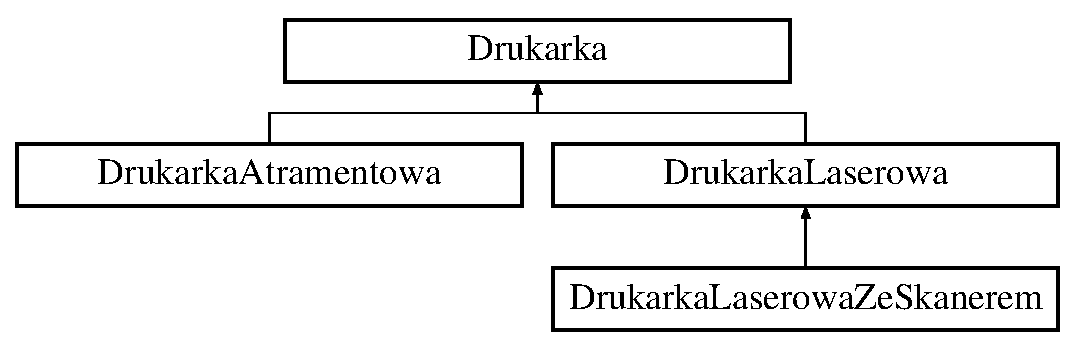
\includegraphics[height=3.000000cm]{class_drukarka}
\end{center}
\end{figure}
\subsection*{Public Member Functions}
\begin{DoxyCompactItemize}
\item 
\textbf{ Drukarka} ()
\begin{DoxyCompactList}\small\item\em Kontruktor domyslny. \end{DoxyCompactList}\item 
virtual \textbf{ $\sim$\+Drukarka} ()
\begin{DoxyCompactList}\small\item\em Destruktor wirtualny. \end{DoxyCompactList}\item 
virtual void \textbf{ zmien\+Parametry\+Urzadzenia} (int nowy\+\_\+parametr)=0
\begin{DoxyCompactList}\small\item\em Zmienna wirtualna. \end{DoxyCompactList}\item 
virtual void \textbf{ wyswietl\+Rodzaj\+Drukarki} ()=0
\begin{DoxyCompactList}\small\item\em Zmienaa wirtualna. \end{DoxyCompactList}\item 
void \textbf{ wyswietl\+Stan} ()
\begin{DoxyCompactList}\small\item\em Funkcja wyswietlajaca stan. \end{DoxyCompactList}\end{DoxyCompactItemize}
\subsection*{Protected Attributes}
\begin{DoxyCompactItemize}
\item 
string \textbf{ stan}
\begin{DoxyCompactList}\small\item\em Zmienna przechowujaca stan. \end{DoxyCompactList}\end{DoxyCompactItemize}
\subsection*{Friends}
\begin{DoxyCompactItemize}
\item 
std\+::ostream \& \textbf{ operator$<$$<$} (std\+::ostream \&d, \textbf{ Drukarka} \&drukarka)
\begin{DoxyCompactList}\small\item\em Operator strumieniowy $<$$<$. \end{DoxyCompactList}\item 
std\+::istream \& \textbf{ operator$>$$>$} (std\+::istream \&d, \textbf{ Drukarka} \&drukarka)
\begin{DoxyCompactList}\small\item\em Operator strumieniowy $>$$>$ \end{DoxyCompactList}\end{DoxyCompactItemize}


\subsection{Detailed Description}
Klasa abstrakcyjna. 

\subsection{Constructor \& Destructor Documentation}
\mbox{\label{class_drukarka_aed4b71f0d650809ea61382a8db8bb41d}} 
\index{Drukarka@{Drukarka}!Drukarka@{Drukarka}}
\index{Drukarka@{Drukarka}!Drukarka@{Drukarka}}
\subsubsection{Drukarka()}
{\footnotesize\ttfamily Drukarka\+::\+Drukarka (\begin{DoxyParamCaption}{ }\end{DoxyParamCaption})}



Kontruktor domyslny. 

\mbox{\label{class_drukarka_a056e3d77c9c294a0870aef831985bd4d}} 
\index{Drukarka@{Drukarka}!````~Drukarka@{$\sim$\+Drukarka}}
\index{````~Drukarka@{$\sim$\+Drukarka}!Drukarka@{Drukarka}}
\subsubsection{$\sim$\+Drukarka()}
{\footnotesize\ttfamily Drukarka\+::$\sim$\+Drukarka (\begin{DoxyParamCaption}{ }\end{DoxyParamCaption})\hspace{0.3cm}{\ttfamily [virtual]}}



Destruktor wirtualny. 



\subsection{Member Function Documentation}
\mbox{\label{class_drukarka_ac31957e9a068dad8dd4a3366885b3aa1}} 
\index{Drukarka@{Drukarka}!wyswietl\+Rodzaj\+Drukarki@{wyswietl\+Rodzaj\+Drukarki}}
\index{wyswietl\+Rodzaj\+Drukarki@{wyswietl\+Rodzaj\+Drukarki}!Drukarka@{Drukarka}}
\subsubsection{wyswietl\+Rodzaj\+Drukarki()}
{\footnotesize\ttfamily virtual void Drukarka\+::wyswietl\+Rodzaj\+Drukarki (\begin{DoxyParamCaption}{ }\end{DoxyParamCaption})\hspace{0.3cm}{\ttfamily [pure virtual]}}



Zmienaa wirtualna. 



Implemented in \textbf{ Drukarka\+Laserowa} \doxyref{}{p.}{class_drukarka_laserowa_a6317c4138c4b0f5f26d7209aa9f6de86}, \textbf{ Drukarka\+Atramentowa} \doxyref{}{p.}{class_drukarka_atramentowa_a178e4ca78646b7dc86431c02952864c1}, and \textbf{ Drukarka\+Laserowa\+Ze\+Skanerem} \doxyref{}{p.}{class_drukarka_laserowa_ze_skanerem_aa37311823ae51a267ab614082ed38162}.

\mbox{\label{class_drukarka_ac79401db16185195592fb64c8b8642aa}} 
\index{Drukarka@{Drukarka}!wyswietl\+Stan@{wyswietl\+Stan}}
\index{wyswietl\+Stan@{wyswietl\+Stan}!Drukarka@{Drukarka}}
\subsubsection{wyswietl\+Stan()}
{\footnotesize\ttfamily void Drukarka\+::wyswietl\+Stan (\begin{DoxyParamCaption}{ }\end{DoxyParamCaption})}



Funkcja wyswietlajaca stan. 

\mbox{\label{class_drukarka_a0c0973a1330f5d20d20f617d7f4ad815}} 
\index{Drukarka@{Drukarka}!zmien\+Parametry\+Urzadzenia@{zmien\+Parametry\+Urzadzenia}}
\index{zmien\+Parametry\+Urzadzenia@{zmien\+Parametry\+Urzadzenia}!Drukarka@{Drukarka}}
\subsubsection{zmien\+Parametry\+Urzadzenia()}
{\footnotesize\ttfamily virtual void Drukarka\+::zmien\+Parametry\+Urzadzenia (\begin{DoxyParamCaption}\item[{int}]{nowy\+\_\+parametr }\end{DoxyParamCaption})\hspace{0.3cm}{\ttfamily [pure virtual]}}



Zmienna wirtualna. 



Implemented in \textbf{ Drukarka\+Laserowa} \doxyref{}{p.}{class_drukarka_laserowa_aeb1c4870b0c7570a99992a694c7aebd1}, \textbf{ Drukarka\+Atramentowa} \doxyref{}{p.}{class_drukarka_atramentowa_acd6bfc005dffc30e57a9106ce175fc7b}, and \textbf{ Drukarka\+Laserowa\+Ze\+Skanerem} \doxyref{}{p.}{class_drukarka_laserowa_ze_skanerem_af32643998dec727591bb3956074800b7}.



\subsection{Friends And Related Function Documentation}
\mbox{\label{class_drukarka_a82275125afd4c7b7e83ea20c28802918}} 
\index{Drukarka@{Drukarka}!operator$<$$<$@{operator$<$$<$}}
\index{operator$<$$<$@{operator$<$$<$}!Drukarka@{Drukarka}}
\subsubsection{operator$<$$<$}
{\footnotesize\ttfamily std\+::ostream\& operator$<$$<$ (\begin{DoxyParamCaption}\item[{std\+::ostream \&}]{d,  }\item[{\textbf{ Drukarka} \&}]{drukarka }\end{DoxyParamCaption})\hspace{0.3cm}{\ttfamily [friend]}}



Operator strumieniowy $<$$<$. 

\mbox{\label{class_drukarka_a690d14a94727eaaeb482b4fa3356c761}} 
\index{Drukarka@{Drukarka}!operator$>$$>$@{operator$>$$>$}}
\index{operator$>$$>$@{operator$>$$>$}!Drukarka@{Drukarka}}
\subsubsection{operator$>$$>$}
{\footnotesize\ttfamily std\+::istream\& operator$>$$>$ (\begin{DoxyParamCaption}\item[{std\+::istream \&}]{d,  }\item[{\textbf{ Drukarka} \&}]{drukarka }\end{DoxyParamCaption})\hspace{0.3cm}{\ttfamily [friend]}}



Operator strumieniowy $>$$>$ 



\subsection{Member Data Documentation}
\mbox{\label{class_drukarka_ade58bac6c2c62bc4cd73ea38a34a0eca}} 
\index{Drukarka@{Drukarka}!stan@{stan}}
\index{stan@{stan}!Drukarka@{Drukarka}}
\subsubsection{stan}
{\footnotesize\ttfamily string Drukarka\+::stan\hspace{0.3cm}{\ttfamily [protected]}}



Zmienna przechowujaca stan. 



The documentation for this class was generated from the following files\+:\begin{DoxyCompactItemize}
\item 
Drukarka\+Laserowa cz.\+2/\textbf{ Drukarka.\+h}\item 
Drukarka\+Laserowa cz.\+2/\textbf{ Drukarka.\+cpp}\end{DoxyCompactItemize}

\section{Drukarka\+Atramentowa Class Reference}
\label{class_drukarka_atramentowa}\index{Drukarka\+Atramentowa@{Drukarka\+Atramentowa}}


Klasa \doxyref{Drukarka\+Atramentowa}{p.}{class_drukarka_atramentowa}, pochodna klasy \doxyref{Drukarka}{p.}{class_drukarka}.  




{\ttfamily \#include $<$Drukarka\+Atramentowa.\+h$>$}

Inheritance diagram for Drukarka\+Atramentowa\+:\begin{figure}[H]
\begin{center}
\leavevmode
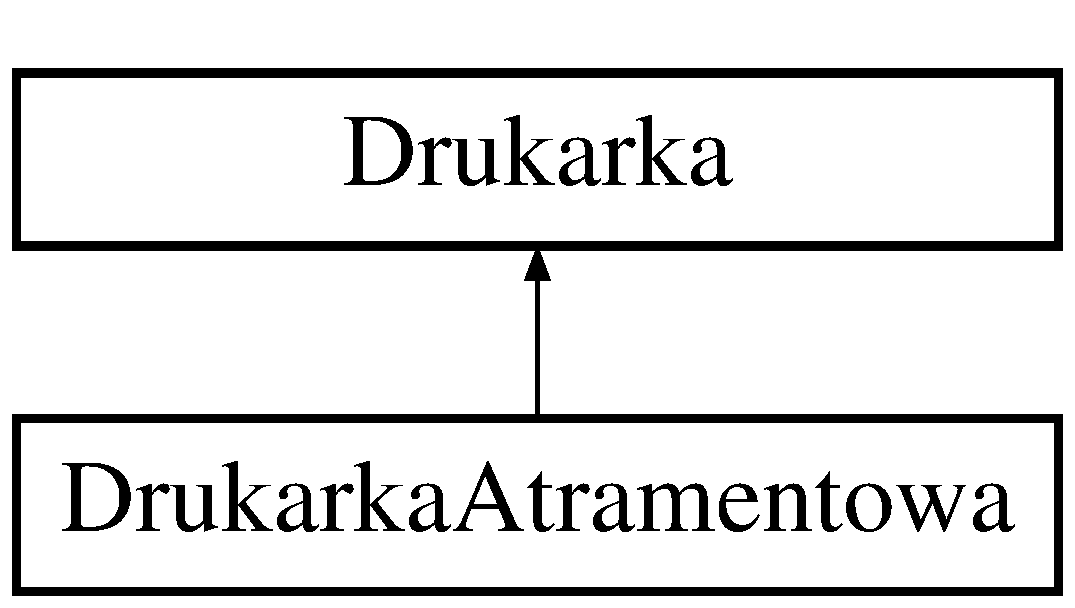
\includegraphics[height=2.000000cm]{class_drukarka_atramentowa}
\end{center}
\end{figure}
\subsection*{Public Member Functions}
\begin{DoxyCompactItemize}
\item 
\textbf{ Drukarka\+Atramentowa} ()
\begin{DoxyCompactList}\small\item\em Kontruktor domyslny. \end{DoxyCompactList}\item 
\textbf{ $\sim$\+Drukarka\+Atramentowa} ()
\begin{DoxyCompactList}\small\item\em Destruktor. \end{DoxyCompactList}\item 
void \textbf{ zmien\+Nazwe} (string \textbf{ nowa\+\_\+nazwa})
\begin{DoxyCompactList}\small\item\em Funkcja modyfikujaca pole nazwy. \end{DoxyCompactList}\item 
void \textbf{ zmien\+Marke} (string \textbf{ nowa\+\_\+marka})
\begin{DoxyCompactList}\small\item\em Funkcja modyfikujaca pole marki. \end{DoxyCompactList}\item 
void \textbf{ wyswietl\+Urzadzenie} ()
\begin{DoxyCompactList}\small\item\em Funkcja wyswietlajaca aktualne urzadzenie. \end{DoxyCompactList}\item 
void \textbf{ wyswietl\+Rodzaj\+Drukarki} ()
\begin{DoxyCompactList}\small\item\em Funkcja wyswietlajaca rodzaj drukarki. \end{DoxyCompactList}\item 
void \textbf{ wyswietl\+Stan} ()
\begin{DoxyCompactList}\small\item\em Funkcja wyswietlajaca stan drukarki. \end{DoxyCompactList}\item 
void \textbf{ zapisz\+Urzadzenie} (\textbf{ Drukarka\+Atramentowa} \&atramentowa)
\begin{DoxyCompactList}\small\item\em Zapisuje aktualne urzadzenie. \end{DoxyCompactList}\item 
void \textbf{ wczytaj\+Urzadzenie} (\textbf{ Drukarka\+Atramentowa} \&atramentowa)
\begin{DoxyCompactList}\small\item\em Wczytuje aktualne urzadzenie. \end{DoxyCompactList}\item 
void \textbf{ zmien\+Parametry\+Urzadzenia} (int nowy\+\_\+parametr)
\begin{DoxyCompactList}\small\item\em Funkcja zmieniajaca wybrany parametr urzadzeni. \end{DoxyCompactList}\end{DoxyCompactItemize}
\subsection*{Protected Attributes}
\begin{DoxyCompactItemize}
\item 
string \textbf{ nazwa}
\begin{DoxyCompactList}\small\item\em Zmienna przechowujaca nazwe drukarki. \end{DoxyCompactList}\item 
string \textbf{ marka}
\begin{DoxyCompactList}\small\item\em Zmienna przechowujaca marke drukarki. \end{DoxyCompactList}\item 
int \textbf{ pamiec\+\_\+wewnetrzna}
\begin{DoxyCompactList}\small\item\em Zmienna przechowujaca pamiec wewnetrzna drukarki. \end{DoxyCompactList}\end{DoxyCompactItemize}
\subsection*{Friends}
\begin{DoxyCompactItemize}
\item 
std\+::ostream \& \textbf{ operator$<$$<$} (std\+::ostream \&a, \textbf{ Drukarka\+Atramentowa} \&atramentowa)
\begin{DoxyCompactList}\small\item\em Operator strumieniowy $<$$<$. \end{DoxyCompactList}\item 
std\+::istream \& \textbf{ operator$>$$>$} (std\+::istream \&a, \textbf{ Drukarka\+Atramentowa} \&atramentowa)
\begin{DoxyCompactList}\small\item\em Operator strumieniowy $>$$>$ \end{DoxyCompactList}\end{DoxyCompactItemize}


\subsection{Detailed Description}
Klasa \doxyref{Drukarka\+Atramentowa}{p.}{class_drukarka_atramentowa}, pochodna klasy \doxyref{Drukarka}{p.}{class_drukarka}. 

\subsection{Constructor \& Destructor Documentation}
\mbox{\label{class_drukarka_atramentowa_af9767e713ce25e354e78d9e0d7854011}} 
\index{Drukarka\+Atramentowa@{Drukarka\+Atramentowa}!Drukarka\+Atramentowa@{Drukarka\+Atramentowa}}
\index{Drukarka\+Atramentowa@{Drukarka\+Atramentowa}!Drukarka\+Atramentowa@{Drukarka\+Atramentowa}}
\subsubsection{Drukarka\+Atramentowa()}
{\footnotesize\ttfamily Drukarka\+Atramentowa\+::\+Drukarka\+Atramentowa (\begin{DoxyParamCaption}{ }\end{DoxyParamCaption})}



Kontruktor domyslny. 

\mbox{\label{class_drukarka_atramentowa_a5294d2f4d2f57bb92fa5b9c7166353e2}} 
\index{Drukarka\+Atramentowa@{Drukarka\+Atramentowa}!````~Drukarka\+Atramentowa@{$\sim$\+Drukarka\+Atramentowa}}
\index{````~Drukarka\+Atramentowa@{$\sim$\+Drukarka\+Atramentowa}!Drukarka\+Atramentowa@{Drukarka\+Atramentowa}}
\subsubsection{$\sim$\+Drukarka\+Atramentowa()}
{\footnotesize\ttfamily Drukarka\+Atramentowa\+::$\sim$\+Drukarka\+Atramentowa (\begin{DoxyParamCaption}{ }\end{DoxyParamCaption})}



Destruktor. 



\subsection{Member Function Documentation}
\mbox{\label{class_drukarka_atramentowa_adf14978278f44b8a7afcea4073db2b94}} 
\index{Drukarka\+Atramentowa@{Drukarka\+Atramentowa}!wczytaj\+Urzadzenie@{wczytaj\+Urzadzenie}}
\index{wczytaj\+Urzadzenie@{wczytaj\+Urzadzenie}!Drukarka\+Atramentowa@{Drukarka\+Atramentowa}}
\subsubsection{wczytaj\+Urzadzenie()}
{\footnotesize\ttfamily void Drukarka\+Atramentowa\+::wczytaj\+Urzadzenie (\begin{DoxyParamCaption}\item[{\textbf{ Drukarka\+Atramentowa} \&}]{atramentowa }\end{DoxyParamCaption})}



Wczytuje aktualne urzadzenie. 

\mbox{\label{class_drukarka_atramentowa_a178e4ca78646b7dc86431c02952864c1}} 
\index{Drukarka\+Atramentowa@{Drukarka\+Atramentowa}!wyswietl\+Rodzaj\+Drukarki@{wyswietl\+Rodzaj\+Drukarki}}
\index{wyswietl\+Rodzaj\+Drukarki@{wyswietl\+Rodzaj\+Drukarki}!Drukarka\+Atramentowa@{Drukarka\+Atramentowa}}
\subsubsection{wyswietl\+Rodzaj\+Drukarki()}
{\footnotesize\ttfamily void Drukarka\+Atramentowa\+::wyswietl\+Rodzaj\+Drukarki (\begin{DoxyParamCaption}{ }\end{DoxyParamCaption})\hspace{0.3cm}{\ttfamily [virtual]}}



Funkcja wyswietlajaca rodzaj drukarki. 



Implements \textbf{ Drukarka} \doxyref{}{p.}{class_drukarka_ac31957e9a068dad8dd4a3366885b3aa1}.

\mbox{\label{class_drukarka_atramentowa_ad1131fef70745264afbeb40e68cbcc93}} 
\index{Drukarka\+Atramentowa@{Drukarka\+Atramentowa}!wyswietl\+Stan@{wyswietl\+Stan}}
\index{wyswietl\+Stan@{wyswietl\+Stan}!Drukarka\+Atramentowa@{Drukarka\+Atramentowa}}
\subsubsection{wyswietl\+Stan()}
{\footnotesize\ttfamily void Drukarka\+Atramentowa\+::wyswietl\+Stan (\begin{DoxyParamCaption}{ }\end{DoxyParamCaption})}



Funkcja wyswietlajaca stan drukarki. 

\mbox{\label{class_drukarka_atramentowa_af10a296b97424fc011bc9016617a5bdc}} 
\index{Drukarka\+Atramentowa@{Drukarka\+Atramentowa}!wyswietl\+Urzadzenie@{wyswietl\+Urzadzenie}}
\index{wyswietl\+Urzadzenie@{wyswietl\+Urzadzenie}!Drukarka\+Atramentowa@{Drukarka\+Atramentowa}}
\subsubsection{wyswietl\+Urzadzenie()}
{\footnotesize\ttfamily void Drukarka\+Atramentowa\+::wyswietl\+Urzadzenie (\begin{DoxyParamCaption}{ }\end{DoxyParamCaption})}



Funkcja wyswietlajaca aktualne urzadzenie. 

\mbox{\label{class_drukarka_atramentowa_a46035be566876f5f433f2c7e9487f7f3}} 
\index{Drukarka\+Atramentowa@{Drukarka\+Atramentowa}!zapisz\+Urzadzenie@{zapisz\+Urzadzenie}}
\index{zapisz\+Urzadzenie@{zapisz\+Urzadzenie}!Drukarka\+Atramentowa@{Drukarka\+Atramentowa}}
\subsubsection{zapisz\+Urzadzenie()}
{\footnotesize\ttfamily void Drukarka\+Atramentowa\+::zapisz\+Urzadzenie (\begin{DoxyParamCaption}\item[{\textbf{ Drukarka\+Atramentowa} \&}]{atramentowa }\end{DoxyParamCaption})}



Zapisuje aktualne urzadzenie. 

\mbox{\label{class_drukarka_atramentowa_aedc85daa45543795f258d3256484bade}} 
\index{Drukarka\+Atramentowa@{Drukarka\+Atramentowa}!zmien\+Marke@{zmien\+Marke}}
\index{zmien\+Marke@{zmien\+Marke}!Drukarka\+Atramentowa@{Drukarka\+Atramentowa}}
\subsubsection{zmien\+Marke()}
{\footnotesize\ttfamily void Drukarka\+Atramentowa\+::zmien\+Marke (\begin{DoxyParamCaption}\item[{string}]{nowa\+\_\+marka }\end{DoxyParamCaption})}



Funkcja modyfikujaca pole marki. 

\mbox{\label{class_drukarka_atramentowa_a5f3d491c41ef7c9781eb606e2f4eb6fb}} 
\index{Drukarka\+Atramentowa@{Drukarka\+Atramentowa}!zmien\+Nazwe@{zmien\+Nazwe}}
\index{zmien\+Nazwe@{zmien\+Nazwe}!Drukarka\+Atramentowa@{Drukarka\+Atramentowa}}
\subsubsection{zmien\+Nazwe()}
{\footnotesize\ttfamily void Drukarka\+Atramentowa\+::zmien\+Nazwe (\begin{DoxyParamCaption}\item[{string}]{nowa\+\_\+nazwa }\end{DoxyParamCaption})}



Funkcja modyfikujaca pole nazwy. 

\mbox{\label{class_drukarka_atramentowa_acd6bfc005dffc30e57a9106ce175fc7b}} 
\index{Drukarka\+Atramentowa@{Drukarka\+Atramentowa}!zmien\+Parametry\+Urzadzenia@{zmien\+Parametry\+Urzadzenia}}
\index{zmien\+Parametry\+Urzadzenia@{zmien\+Parametry\+Urzadzenia}!Drukarka\+Atramentowa@{Drukarka\+Atramentowa}}
\subsubsection{zmien\+Parametry\+Urzadzenia()}
{\footnotesize\ttfamily void Drukarka\+Atramentowa\+::zmien\+Parametry\+Urzadzenia (\begin{DoxyParamCaption}\item[{int}]{nowy\+\_\+parametr }\end{DoxyParamCaption})\hspace{0.3cm}{\ttfamily [virtual]}}



Funkcja zmieniajaca wybrany parametr urzadzeni. 



Implements \textbf{ Drukarka} \doxyref{}{p.}{class_drukarka_a0c0973a1330f5d20d20f617d7f4ad815}.



\subsection{Friends And Related Function Documentation}
\mbox{\label{class_drukarka_atramentowa_ad64f242b639e39ead86b549a16794760}} 
\index{Drukarka\+Atramentowa@{Drukarka\+Atramentowa}!operator$<$$<$@{operator$<$$<$}}
\index{operator$<$$<$@{operator$<$$<$}!Drukarka\+Atramentowa@{Drukarka\+Atramentowa}}
\subsubsection{operator$<$$<$}
{\footnotesize\ttfamily std\+::ostream\& operator$<$$<$ (\begin{DoxyParamCaption}\item[{std\+::ostream \&}]{a,  }\item[{\textbf{ Drukarka\+Atramentowa} \&}]{atramentowa }\end{DoxyParamCaption})\hspace{0.3cm}{\ttfamily [friend]}}



Operator strumieniowy $<$$<$. 

\mbox{\label{class_drukarka_atramentowa_ad81030cdd68ff1bd6990456164f9fe44}} 
\index{Drukarka\+Atramentowa@{Drukarka\+Atramentowa}!operator$>$$>$@{operator$>$$>$}}
\index{operator$>$$>$@{operator$>$$>$}!Drukarka\+Atramentowa@{Drukarka\+Atramentowa}}
\subsubsection{operator$>$$>$}
{\footnotesize\ttfamily std\+::istream\& operator$>$$>$ (\begin{DoxyParamCaption}\item[{std\+::istream \&}]{a,  }\item[{\textbf{ Drukarka\+Atramentowa} \&}]{atramentowa }\end{DoxyParamCaption})\hspace{0.3cm}{\ttfamily [friend]}}



Operator strumieniowy $>$$>$ 



\subsection{Member Data Documentation}
\mbox{\label{class_drukarka_atramentowa_a70c4fe13a56744d291af7ee896842418}} 
\index{Drukarka\+Atramentowa@{Drukarka\+Atramentowa}!marka@{marka}}
\index{marka@{marka}!Drukarka\+Atramentowa@{Drukarka\+Atramentowa}}
\subsubsection{marka}
{\footnotesize\ttfamily string Drukarka\+Atramentowa\+::marka\hspace{0.3cm}{\ttfamily [protected]}}



Zmienna przechowujaca marke drukarki. 

\mbox{\label{class_drukarka_atramentowa_a8cf00dee944e45ccd01e385d27368589}} 
\index{Drukarka\+Atramentowa@{Drukarka\+Atramentowa}!nazwa@{nazwa}}
\index{nazwa@{nazwa}!Drukarka\+Atramentowa@{Drukarka\+Atramentowa}}
\subsubsection{nazwa}
{\footnotesize\ttfamily string Drukarka\+Atramentowa\+::nazwa\hspace{0.3cm}{\ttfamily [protected]}}



Zmienna przechowujaca nazwe drukarki. 

\mbox{\label{class_drukarka_atramentowa_a8480b700e689e211e2f70329608c35eb}} 
\index{Drukarka\+Atramentowa@{Drukarka\+Atramentowa}!pamiec\+\_\+wewnetrzna@{pamiec\+\_\+wewnetrzna}}
\index{pamiec\+\_\+wewnetrzna@{pamiec\+\_\+wewnetrzna}!Drukarka\+Atramentowa@{Drukarka\+Atramentowa}}
\subsubsection{pamiec\+\_\+wewnetrzna}
{\footnotesize\ttfamily int Drukarka\+Atramentowa\+::pamiec\+\_\+wewnetrzna\hspace{0.3cm}{\ttfamily [protected]}}



Zmienna przechowujaca pamiec wewnetrzna drukarki. 



The documentation for this class was generated from the following files\+:\begin{DoxyCompactItemize}
\item 
Drukarka\+Laserowa cz.\+2/\textbf{ Drukarka\+Atramentowa.\+h}\item 
Drukarka\+Laserowa cz.\+2/\textbf{ Drukarka\+Atramentowa.\+cpp}\end{DoxyCompactItemize}

\section{Drukarka\+Laserowa Class Reference}
\label{class_drukarka_laserowa}\index{Drukarka\+Laserowa@{Drukarka\+Laserowa}}


Klasa \doxyref{Drukarka\+Laserowa}{p.}{class_drukarka_laserowa}, pochodna klasy \doxyref{Drukarka}{p.}{class_drukarka}.  




{\ttfamily \#include $<$Drukarka\+Laserowa.\+h$>$}

Inheritance diagram for Drukarka\+Laserowa\+:\begin{figure}[H]
\begin{center}
\leavevmode
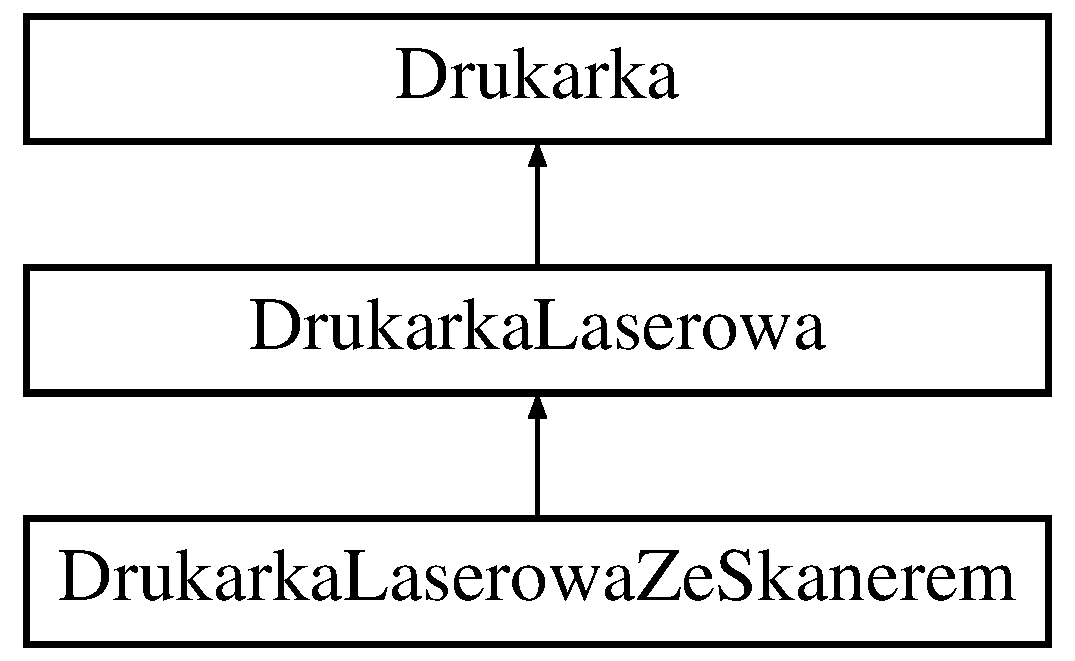
\includegraphics[height=3.000000cm]{class_drukarka_laserowa}
\end{center}
\end{figure}
\subsection*{Public Member Functions}
\begin{DoxyCompactItemize}
\item 
\textbf{ Drukarka\+Laserowa} ()
\begin{DoxyCompactList}\small\item\em Kontruktor domyslny. \end{DoxyCompactList}\item 
\textbf{ Drukarka\+Laserowa} (int pamiec)
\begin{DoxyCompactList}\small\item\em Konstruktor. \end{DoxyCompactList}\item 
\textbf{ $\sim$\+Drukarka\+Laserowa} ()
\begin{DoxyCompactList}\small\item\em Destruktor. \end{DoxyCompactList}\item 
\textbf{ Drukarka\+Laserowa} (const \textbf{ Drukarka\+Laserowa} \&drukarka\+\_\+laserowa)
\begin{DoxyCompactList}\small\item\em Konstruktor kopiujacy. \end{DoxyCompactList}\item 
void \textbf{ zmien\+Nazwe} (string \textbf{ nowa\+\_\+nazwa})
\begin{DoxyCompactList}\small\item\em Funkcja modyfikujaca pole nazwy. \end{DoxyCompactList}\item 
void \textbf{ zmien\+Marke} (string \textbf{ nowa\+\_\+marka})
\begin{DoxyCompactList}\small\item\em Funkcja modyfikujaca pole marki. \end{DoxyCompactList}\item 
void \textbf{ wyswietl\+Urzadzenie} ()
\begin{DoxyCompactList}\small\item\em Funkcja wyswietlajaca aktualne urzadzenie. \end{DoxyCompactList}\item 
void \textbf{ wyswietl\+Rodzaj\+Drukarki} ()
\begin{DoxyCompactList}\small\item\em Funkcja wyswietlajaca rodzaj drukarki. \end{DoxyCompactList}\item 
void \textbf{ wyswietl\+Ilosc} ()
\begin{DoxyCompactList}\small\item\em Funkcja Wyswietlajaca ilsc stworzonych obiektow. \end{DoxyCompactList}\item 
void \textbf{ zapisz\+Urzadzenie} (\textbf{ Drukarka\+Laserowa} \&drukarka\+\_\+laserowa)
\begin{DoxyCompactList}\small\item\em Zapisuje aktualne urzadzenie. \end{DoxyCompactList}\item 
void \textbf{ wczytaj\+Urzadzenie} (\textbf{ Drukarka\+Laserowa} \&drukarka\+\_\+laserowa)
\begin{DoxyCompactList}\small\item\em Wczytuje aktualne urzadzenie. \end{DoxyCompactList}\item 
void \textbf{ zmien\+Parametry\+Urzadzenia} (int nowy\+\_\+parametr)
\begin{DoxyCompactList}\small\item\em Funkcja zmieniajaca wybrany parametr urzadzeni. \end{DoxyCompactList}\item 
void \textbf{ wyswietl\+Stan} ()
\begin{DoxyCompactList}\small\item\em Funkcja wyswietlajaca stan drukarki. \end{DoxyCompactList}\item 
bool \textbf{ operator==} (const \textbf{ Drukarka\+Laserowa} \&drukarka\+\_\+laserowa)
\begin{DoxyCompactList}\small\item\em operator == \end{DoxyCompactList}\item 
bool \textbf{ operator$>$} (const \textbf{ Drukarka\+Laserowa} \&drukarka\+\_\+laserowa)
\begin{DoxyCompactList}\small\item\em operator $>$ \end{DoxyCompactList}\item 
bool \textbf{ operator$<$} (const \textbf{ Drukarka\+Laserowa} \&drukarka\+\_\+laserowa)
\begin{DoxyCompactList}\small\item\em operator $<$ \end{DoxyCompactList}\item 
\textbf{ Drukarka\+Laserowa} \& \textbf{ operator=} (const \textbf{ Drukarka\+Laserowa} \&drukarka\+\_\+laserowa)
\begin{DoxyCompactList}\small\item\em operator = \end{DoxyCompactList}\item 
\textbf{ Drukarka\+Laserowa} \textbf{ operator+} (const \textbf{ Drukarka\+Laserowa} \&drukarka\+\_\+laserowa)
\begin{DoxyCompactList}\small\item\em operator + \end{DoxyCompactList}\item 
\textbf{ Drukarka\+Laserowa} \textbf{ operator$\ast$} (const \textbf{ Drukarka\+Laserowa} \&drukarka\+\_\+laserowa)
\begin{DoxyCompactList}\small\item\em operator $\ast$ \end{DoxyCompactList}\item 
\textbf{ Drukarka\+Laserowa} \& \textbf{ operator+=} (const \textbf{ Drukarka\+Laserowa} \&drukarka\+\_\+laserowa)
\begin{DoxyCompactList}\small\item\em operator += \end{DoxyCompactList}\item 
\textbf{ Drukarka\+Laserowa} \& \textbf{ operator-\/=} (const \textbf{ Drukarka\+Laserowa} \&drukarka\+\_\+laserowa)
\begin{DoxyCompactList}\small\item\em operator -\/= \end{DoxyCompactList}\item 
\textbf{ Drukarka\+Laserowa} \& \textbf{ operator++} (int)
\begin{DoxyCompactList}\small\item\em operator ++ \end{DoxyCompactList}\item 
\textbf{ Drukarka\+Laserowa} \& \textbf{ operator-\/-\/} (int)
\begin{DoxyCompactList}\small\item\em operator -- \end{DoxyCompactList}\end{DoxyCompactItemize}
\subsection*{Protected Attributes}
\begin{DoxyCompactItemize}
\item 
string \textbf{ nazwa}
\begin{DoxyCompactList}\small\item\em Zmienna przechowujaca nazwe drukarki. \end{DoxyCompactList}\item 
string \textbf{ marka}
\begin{DoxyCompactList}\small\item\em Zmienna przechowujaca marke drukarki. \end{DoxyCompactList}\item 
int \textbf{ pamiec\+\_\+wewnetrzna}
\begin{DoxyCompactList}\small\item\em Zmienna przechowujaca pamiec wewnetrzna drukarki. \end{DoxyCompactList}\end{DoxyCompactItemize}
\subsection*{Static Protected Attributes}
\begin{DoxyCompactItemize}
\item 
static int \textbf{ liczba\+\_\+obiektow} = 0
\begin{DoxyCompactList}\small\item\em Zmienna statyczna, przechowujaca liczbe utworzonych obiektow. \end{DoxyCompactList}\end{DoxyCompactItemize}
\subsection*{Friends}
\begin{DoxyCompactItemize}
\item 
std\+::ostream \& \textbf{ operator$<$$<$} (std\+::ostream \&l, \textbf{ Drukarka\+Laserowa} \&drukarka\+\_\+laserowa)
\begin{DoxyCompactList}\small\item\em Operator strumieniowy $<$$<$. \end{DoxyCompactList}\item 
std\+::istream \& \textbf{ operator$>$$>$} (std\+::istream \&l, \textbf{ Drukarka\+Laserowa} \&drukarka\+\_\+laserowa)
\begin{DoxyCompactList}\small\item\em Operator strumieniowy $>$$>$ \end{DoxyCompactList}\end{DoxyCompactItemize}


\subsection{Detailed Description}
Klasa \doxyref{Drukarka\+Laserowa}{p.}{class_drukarka_laserowa}, pochodna klasy \doxyref{Drukarka}{p.}{class_drukarka}. 

\subsection{Constructor \& Destructor Documentation}
\mbox{\label{class_drukarka_laserowa_a7f541671aab057fa95c4726d9c6bc176}} 
\index{Drukarka\+Laserowa@{Drukarka\+Laserowa}!Drukarka\+Laserowa@{Drukarka\+Laserowa}}
\index{Drukarka\+Laserowa@{Drukarka\+Laserowa}!Drukarka\+Laserowa@{Drukarka\+Laserowa}}
\subsubsection{Drukarka\+Laserowa()\hspace{0.1cm}{\footnotesize\ttfamily [1/3]}}
{\footnotesize\ttfamily Drukarka\+Laserowa\+::\+Drukarka\+Laserowa (\begin{DoxyParamCaption}{ }\end{DoxyParamCaption})}



Kontruktor domyslny. 

\mbox{\label{class_drukarka_laserowa_afec2369af7041f4e9311a33d10a87809}} 
\index{Drukarka\+Laserowa@{Drukarka\+Laserowa}!Drukarka\+Laserowa@{Drukarka\+Laserowa}}
\index{Drukarka\+Laserowa@{Drukarka\+Laserowa}!Drukarka\+Laserowa@{Drukarka\+Laserowa}}
\subsubsection{Drukarka\+Laserowa()\hspace{0.1cm}{\footnotesize\ttfamily [2/3]}}
{\footnotesize\ttfamily Drukarka\+Laserowa\+::\+Drukarka\+Laserowa (\begin{DoxyParamCaption}\item[{int}]{pamiec }\end{DoxyParamCaption})}



Konstruktor. 

\mbox{\label{class_drukarka_laserowa_a73ac561ef9e6375782799fa8035487df}} 
\index{Drukarka\+Laserowa@{Drukarka\+Laserowa}!````~Drukarka\+Laserowa@{$\sim$\+Drukarka\+Laserowa}}
\index{````~Drukarka\+Laserowa@{$\sim$\+Drukarka\+Laserowa}!Drukarka\+Laserowa@{Drukarka\+Laserowa}}
\subsubsection{$\sim$\+Drukarka\+Laserowa()}
{\footnotesize\ttfamily Drukarka\+Laserowa\+::$\sim$\+Drukarka\+Laserowa (\begin{DoxyParamCaption}{ }\end{DoxyParamCaption})}



Destruktor. 

\mbox{\label{class_drukarka_laserowa_a3e057d583745023e4bfe78adb1b68e58}} 
\index{Drukarka\+Laserowa@{Drukarka\+Laserowa}!Drukarka\+Laserowa@{Drukarka\+Laserowa}}
\index{Drukarka\+Laserowa@{Drukarka\+Laserowa}!Drukarka\+Laserowa@{Drukarka\+Laserowa}}
\subsubsection{Drukarka\+Laserowa()\hspace{0.1cm}{\footnotesize\ttfamily [3/3]}}
{\footnotesize\ttfamily Drukarka\+Laserowa\+::\+Drukarka\+Laserowa (\begin{DoxyParamCaption}\item[{const \textbf{ Drukarka\+Laserowa} \&}]{drukarka\+\_\+laserowa }\end{DoxyParamCaption})}



Konstruktor kopiujacy. 



\subsection{Member Function Documentation}
\mbox{\label{class_drukarka_laserowa_abb2ef635ed06ccacf5463492eb716a04}} 
\index{Drukarka\+Laserowa@{Drukarka\+Laserowa}!operator$\ast$@{operator$\ast$}}
\index{operator$\ast$@{operator$\ast$}!Drukarka\+Laserowa@{Drukarka\+Laserowa}}
\subsubsection{operator$\ast$()}
{\footnotesize\ttfamily \textbf{ Drukarka\+Laserowa} Drukarka\+Laserowa\+::operator$\ast$ (\begin{DoxyParamCaption}\item[{const \textbf{ Drukarka\+Laserowa} \&}]{drukarka\+\_\+laserowa }\end{DoxyParamCaption})}



operator $\ast$ 

Operator $\ast$. \mbox{\label{class_drukarka_laserowa_aab711b7b11f29e0add1c4073b52cc249}} 
\index{Drukarka\+Laserowa@{Drukarka\+Laserowa}!operator+@{operator+}}
\index{operator+@{operator+}!Drukarka\+Laserowa@{Drukarka\+Laserowa}}
\subsubsection{operator+()}
{\footnotesize\ttfamily \textbf{ Drukarka\+Laserowa} Drukarka\+Laserowa\+::operator+ (\begin{DoxyParamCaption}\item[{const \textbf{ Drukarka\+Laserowa} \&}]{drukarka\+\_\+laserowa }\end{DoxyParamCaption})}



operator + 

Operator +. \mbox{\label{class_drukarka_laserowa_a5c5721e31cb5d27515d8f7139331ebd7}} 
\index{Drukarka\+Laserowa@{Drukarka\+Laserowa}!operator++@{operator++}}
\index{operator++@{operator++}!Drukarka\+Laserowa@{Drukarka\+Laserowa}}
\subsubsection{operator++()}
{\footnotesize\ttfamily \textbf{ Drukarka\+Laserowa} \& Drukarka\+Laserowa\+::operator++ (\begin{DoxyParamCaption}\item[{int}]{ }\end{DoxyParamCaption})}



operator ++ 

Operator ++. \mbox{\label{class_drukarka_laserowa_a0d46c5eb3ab53b4c5c8fd93d8dd6543b}} 
\index{Drukarka\+Laserowa@{Drukarka\+Laserowa}!operator+=@{operator+=}}
\index{operator+=@{operator+=}!Drukarka\+Laserowa@{Drukarka\+Laserowa}}
\subsubsection{operator+=()}
{\footnotesize\ttfamily \textbf{ Drukarka\+Laserowa} \& Drukarka\+Laserowa\+::operator+= (\begin{DoxyParamCaption}\item[{const \textbf{ Drukarka\+Laserowa} \&}]{drukarka\+\_\+laserowa }\end{DoxyParamCaption})}



operator += 

Operator +=. \mbox{\label{class_drukarka_laserowa_a844daae7f1d6289c8d0b7131567cc48f}} 
\index{Drukarka\+Laserowa@{Drukarka\+Laserowa}!operator-\/-\/@{operator-\/-\/}}
\index{operator-\/-\/@{operator-\/-\/}!Drukarka\+Laserowa@{Drukarka\+Laserowa}}
\subsubsection{operator-\/-\/()}
{\footnotesize\ttfamily \textbf{ Drukarka\+Laserowa} \& Drukarka\+Laserowa\+::operator-\/-\/ (\begin{DoxyParamCaption}\item[{int}]{ }\end{DoxyParamCaption})}



operator -- 

Operator --. \mbox{\label{class_drukarka_laserowa_a48d35026935f191fa5997fb793c73ec4}} 
\index{Drukarka\+Laserowa@{Drukarka\+Laserowa}!operator-\/=@{operator-\/=}}
\index{operator-\/=@{operator-\/=}!Drukarka\+Laserowa@{Drukarka\+Laserowa}}
\subsubsection{operator-\/=()}
{\footnotesize\ttfamily \textbf{ Drukarka\+Laserowa} \& Drukarka\+Laserowa\+::operator-\/= (\begin{DoxyParamCaption}\item[{const \textbf{ Drukarka\+Laserowa} \&}]{drukarka\+\_\+laserowa }\end{DoxyParamCaption})}



operator -\/= 

Operator -\/=. \mbox{\label{class_drukarka_laserowa_af216f092a8f12e6aa9f8cab044e8b362}} 
\index{Drukarka\+Laserowa@{Drukarka\+Laserowa}!operator$<$@{operator$<$}}
\index{operator$<$@{operator$<$}!Drukarka\+Laserowa@{Drukarka\+Laserowa}}
\subsubsection{operator$<$()}
{\footnotesize\ttfamily bool Drukarka\+Laserowa\+::operator$<$ (\begin{DoxyParamCaption}\item[{const \textbf{ Drukarka\+Laserowa} \&}]{drukarka\+\_\+laserowa }\end{DoxyParamCaption})}



operator $<$ 

Operator $<$. \mbox{\label{class_drukarka_laserowa_a898f6d57db0f0870bfbee13b7b1bf401}} 
\index{Drukarka\+Laserowa@{Drukarka\+Laserowa}!operator=@{operator=}}
\index{operator=@{operator=}!Drukarka\+Laserowa@{Drukarka\+Laserowa}}
\subsubsection{operator=()}
{\footnotesize\ttfamily \textbf{ Drukarka\+Laserowa} \& Drukarka\+Laserowa\+::operator= (\begin{DoxyParamCaption}\item[{const \textbf{ Drukarka\+Laserowa} \&}]{drukarka\+\_\+laserowa }\end{DoxyParamCaption})}



operator = 

Operator =. \mbox{\label{class_drukarka_laserowa_ae739d225550a0d69a96d3940f30048cc}} 
\index{Drukarka\+Laserowa@{Drukarka\+Laserowa}!operator==@{operator==}}
\index{operator==@{operator==}!Drukarka\+Laserowa@{Drukarka\+Laserowa}}
\subsubsection{operator==()}
{\footnotesize\ttfamily bool Drukarka\+Laserowa\+::operator== (\begin{DoxyParamCaption}\item[{const \textbf{ Drukarka\+Laserowa} \&}]{drukarka\+\_\+laserowa }\end{DoxyParamCaption})}



operator == 

Operator =. \mbox{\label{class_drukarka_laserowa_ab1cd6a654da9e5ca44cfd49f0e6bb735}} 
\index{Drukarka\+Laserowa@{Drukarka\+Laserowa}!operator$>$@{operator$>$}}
\index{operator$>$@{operator$>$}!Drukarka\+Laserowa@{Drukarka\+Laserowa}}
\subsubsection{operator$>$()}
{\footnotesize\ttfamily bool Drukarka\+Laserowa\+::operator$>$ (\begin{DoxyParamCaption}\item[{const \textbf{ Drukarka\+Laserowa} \&}]{drukarka\+\_\+laserowa }\end{DoxyParamCaption})}



operator $>$ 

Operator $>$ \mbox{\label{class_drukarka_laserowa_aca98bc314c587b60d079d4e909a0c4e4}} 
\index{Drukarka\+Laserowa@{Drukarka\+Laserowa}!wczytaj\+Urzadzenie@{wczytaj\+Urzadzenie}}
\index{wczytaj\+Urzadzenie@{wczytaj\+Urzadzenie}!Drukarka\+Laserowa@{Drukarka\+Laserowa}}
\subsubsection{wczytaj\+Urzadzenie()}
{\footnotesize\ttfamily void Drukarka\+Laserowa\+::wczytaj\+Urzadzenie (\begin{DoxyParamCaption}\item[{\textbf{ Drukarka\+Laserowa} \&}]{drukarka\+\_\+laserowa }\end{DoxyParamCaption})}



Wczytuje aktualne urzadzenie. 

\mbox{\label{class_drukarka_laserowa_ad29f80de9e2a5944f64c72472ab8470e}} 
\index{Drukarka\+Laserowa@{Drukarka\+Laserowa}!wyswietl\+Ilosc@{wyswietl\+Ilosc}}
\index{wyswietl\+Ilosc@{wyswietl\+Ilosc}!Drukarka\+Laserowa@{Drukarka\+Laserowa}}
\subsubsection{wyswietl\+Ilosc()}
{\footnotesize\ttfamily void Drukarka\+Laserowa\+::wyswietl\+Ilosc (\begin{DoxyParamCaption}{ }\end{DoxyParamCaption})}



Funkcja Wyswietlajaca ilsc stworzonych obiektow. 

\mbox{\label{class_drukarka_laserowa_a6317c4138c4b0f5f26d7209aa9f6de86}} 
\index{Drukarka\+Laserowa@{Drukarka\+Laserowa}!wyswietl\+Rodzaj\+Drukarki@{wyswietl\+Rodzaj\+Drukarki}}
\index{wyswietl\+Rodzaj\+Drukarki@{wyswietl\+Rodzaj\+Drukarki}!Drukarka\+Laserowa@{Drukarka\+Laserowa}}
\subsubsection{wyswietl\+Rodzaj\+Drukarki()}
{\footnotesize\ttfamily void Drukarka\+Laserowa\+::wyswietl\+Rodzaj\+Drukarki (\begin{DoxyParamCaption}{ }\end{DoxyParamCaption})\hspace{0.3cm}{\ttfamily [virtual]}}



Funkcja wyswietlajaca rodzaj drukarki. 



Implements \textbf{ Drukarka} \doxyref{}{p.}{class_drukarka_ac31957e9a068dad8dd4a3366885b3aa1}.



Reimplemented in \textbf{ Drukarka\+Laserowa\+Ze\+Skanerem} \doxyref{}{p.}{class_drukarka_laserowa_ze_skanerem_aa37311823ae51a267ab614082ed38162}.

\mbox{\label{class_drukarka_laserowa_a546955bfc3bb343cc828fc4c6624840a}} 
\index{Drukarka\+Laserowa@{Drukarka\+Laserowa}!wyswietl\+Stan@{wyswietl\+Stan}}
\index{wyswietl\+Stan@{wyswietl\+Stan}!Drukarka\+Laserowa@{Drukarka\+Laserowa}}
\subsubsection{wyswietl\+Stan()}
{\footnotesize\ttfamily void Drukarka\+Laserowa\+::wyswietl\+Stan (\begin{DoxyParamCaption}{ }\end{DoxyParamCaption})}



Funkcja wyswietlajaca stan drukarki. 

\mbox{\label{class_drukarka_laserowa_ad101e0282808db040d4d010e497a64e6}} 
\index{Drukarka\+Laserowa@{Drukarka\+Laserowa}!wyswietl\+Urzadzenie@{wyswietl\+Urzadzenie}}
\index{wyswietl\+Urzadzenie@{wyswietl\+Urzadzenie}!Drukarka\+Laserowa@{Drukarka\+Laserowa}}
\subsubsection{wyswietl\+Urzadzenie()}
{\footnotesize\ttfamily void Drukarka\+Laserowa\+::wyswietl\+Urzadzenie (\begin{DoxyParamCaption}{ }\end{DoxyParamCaption})}



Funkcja wyswietlajaca aktualne urzadzenie. 

\mbox{\label{class_drukarka_laserowa_aab5a4c15080963ce1289453d28deb322}} 
\index{Drukarka\+Laserowa@{Drukarka\+Laserowa}!zapisz\+Urzadzenie@{zapisz\+Urzadzenie}}
\index{zapisz\+Urzadzenie@{zapisz\+Urzadzenie}!Drukarka\+Laserowa@{Drukarka\+Laserowa}}
\subsubsection{zapisz\+Urzadzenie()}
{\footnotesize\ttfamily void Drukarka\+Laserowa\+::zapisz\+Urzadzenie (\begin{DoxyParamCaption}\item[{\textbf{ Drukarka\+Laserowa} \&}]{drukarka\+\_\+laserowa }\end{DoxyParamCaption})}



Zapisuje aktualne urzadzenie. 

\mbox{\label{class_drukarka_laserowa_a7af3f3cd2d8a947a3f64de13985706b1}} 
\index{Drukarka\+Laserowa@{Drukarka\+Laserowa}!zmien\+Marke@{zmien\+Marke}}
\index{zmien\+Marke@{zmien\+Marke}!Drukarka\+Laserowa@{Drukarka\+Laserowa}}
\subsubsection{zmien\+Marke()}
{\footnotesize\ttfamily void Drukarka\+Laserowa\+::zmien\+Marke (\begin{DoxyParamCaption}\item[{string}]{nowa\+\_\+marka }\end{DoxyParamCaption})}



Funkcja modyfikujaca pole marki. 

\mbox{\label{class_drukarka_laserowa_a5fed946210dce136b7203172c215df5e}} 
\index{Drukarka\+Laserowa@{Drukarka\+Laserowa}!zmien\+Nazwe@{zmien\+Nazwe}}
\index{zmien\+Nazwe@{zmien\+Nazwe}!Drukarka\+Laserowa@{Drukarka\+Laserowa}}
\subsubsection{zmien\+Nazwe()}
{\footnotesize\ttfamily void Drukarka\+Laserowa\+::zmien\+Nazwe (\begin{DoxyParamCaption}\item[{string}]{nowa\+\_\+nazwa }\end{DoxyParamCaption})}



Funkcja modyfikujaca pole nazwy. 

\mbox{\label{class_drukarka_laserowa_aeb1c4870b0c7570a99992a694c7aebd1}} 
\index{Drukarka\+Laserowa@{Drukarka\+Laserowa}!zmien\+Parametry\+Urzadzenia@{zmien\+Parametry\+Urzadzenia}}
\index{zmien\+Parametry\+Urzadzenia@{zmien\+Parametry\+Urzadzenia}!Drukarka\+Laserowa@{Drukarka\+Laserowa}}
\subsubsection{zmien\+Parametry\+Urzadzenia()}
{\footnotesize\ttfamily void Drukarka\+Laserowa\+::zmien\+Parametry\+Urzadzenia (\begin{DoxyParamCaption}\item[{int}]{nowy\+\_\+parametr }\end{DoxyParamCaption})\hspace{0.3cm}{\ttfamily [virtual]}}



Funkcja zmieniajaca wybrany parametr urzadzeni. 



Implements \textbf{ Drukarka} \doxyref{}{p.}{class_drukarka_a0c0973a1330f5d20d20f617d7f4ad815}.



Reimplemented in \textbf{ Drukarka\+Laserowa\+Ze\+Skanerem} \doxyref{}{p.}{class_drukarka_laserowa_ze_skanerem_af32643998dec727591bb3956074800b7}.



\subsection{Friends And Related Function Documentation}
\mbox{\label{class_drukarka_laserowa_a9aeecb5f56f3f86716b4668ba91803b9}} 
\index{Drukarka\+Laserowa@{Drukarka\+Laserowa}!operator$<$$<$@{operator$<$$<$}}
\index{operator$<$$<$@{operator$<$$<$}!Drukarka\+Laserowa@{Drukarka\+Laserowa}}
\subsubsection{operator$<$$<$}
{\footnotesize\ttfamily std\+::ostream\& operator$<$$<$ (\begin{DoxyParamCaption}\item[{std\+::ostream \&}]{l,  }\item[{\textbf{ Drukarka\+Laserowa} \&}]{drukarka\+\_\+laserowa }\end{DoxyParamCaption})\hspace{0.3cm}{\ttfamily [friend]}}



Operator strumieniowy $<$$<$. 

\mbox{\label{class_drukarka_laserowa_adab561874dc824b55c9695dd73b4cdff}} 
\index{Drukarka\+Laserowa@{Drukarka\+Laserowa}!operator$>$$>$@{operator$>$$>$}}
\index{operator$>$$>$@{operator$>$$>$}!Drukarka\+Laserowa@{Drukarka\+Laserowa}}
\subsubsection{operator$>$$>$}
{\footnotesize\ttfamily std\+::istream\& operator$>$$>$ (\begin{DoxyParamCaption}\item[{std\+::istream \&}]{l,  }\item[{\textbf{ Drukarka\+Laserowa} \&}]{drukarka\+\_\+laserowa }\end{DoxyParamCaption})\hspace{0.3cm}{\ttfamily [friend]}}



Operator strumieniowy $>$$>$ 



\subsection{Member Data Documentation}
\mbox{\label{class_drukarka_laserowa_a6db0507e8fa11025963921d25f40d5b5}} 
\index{Drukarka\+Laserowa@{Drukarka\+Laserowa}!liczba\+\_\+obiektow@{liczba\+\_\+obiektow}}
\index{liczba\+\_\+obiektow@{liczba\+\_\+obiektow}!Drukarka\+Laserowa@{Drukarka\+Laserowa}}
\subsubsection{liczba\+\_\+obiektow}
{\footnotesize\ttfamily int Drukarka\+Laserowa\+::liczba\+\_\+obiektow = 0\hspace{0.3cm}{\ttfamily [static]}, {\ttfamily [protected]}}



Zmienna statyczna, przechowujaca liczbe utworzonych obiektow. 

\mbox{\label{class_drukarka_laserowa_af08d8f7271bed5653b7e297dd79c633b}} 
\index{Drukarka\+Laserowa@{Drukarka\+Laserowa}!marka@{marka}}
\index{marka@{marka}!Drukarka\+Laserowa@{Drukarka\+Laserowa}}
\subsubsection{marka}
{\footnotesize\ttfamily string Drukarka\+Laserowa\+::marka\hspace{0.3cm}{\ttfamily [protected]}}



Zmienna przechowujaca marke drukarki. 

\mbox{\label{class_drukarka_laserowa_ac01f229c688d0c211048471553b200ab}} 
\index{Drukarka\+Laserowa@{Drukarka\+Laserowa}!nazwa@{nazwa}}
\index{nazwa@{nazwa}!Drukarka\+Laserowa@{Drukarka\+Laserowa}}
\subsubsection{nazwa}
{\footnotesize\ttfamily string Drukarka\+Laserowa\+::nazwa\hspace{0.3cm}{\ttfamily [protected]}}



Zmienna przechowujaca nazwe drukarki. 

\mbox{\label{class_drukarka_laserowa_a0f05728fd1a9ad05db2e3e9dbe425dbe}} 
\index{Drukarka\+Laserowa@{Drukarka\+Laserowa}!pamiec\+\_\+wewnetrzna@{pamiec\+\_\+wewnetrzna}}
\index{pamiec\+\_\+wewnetrzna@{pamiec\+\_\+wewnetrzna}!Drukarka\+Laserowa@{Drukarka\+Laserowa}}
\subsubsection{pamiec\+\_\+wewnetrzna}
{\footnotesize\ttfamily int Drukarka\+Laserowa\+::pamiec\+\_\+wewnetrzna\hspace{0.3cm}{\ttfamily [protected]}}



Zmienna przechowujaca pamiec wewnetrzna drukarki. 



The documentation for this class was generated from the following files\+:\begin{DoxyCompactItemize}
\item 
Drukarka\+Laserowa cz.\+2/\textbf{ Drukarka\+Laserowa.\+h}\item 
Drukarka\+Laserowa cz.\+2/\textbf{ Drukarka\+Laserowa.\+cpp}\end{DoxyCompactItemize}

\section{Drukarka\+Laserowa\+Ze\+Skanerem Class Reference}
\label{class_drukarka_laserowa_ze_skanerem}\index{Drukarka\+Laserowa\+Ze\+Skanerem@{Drukarka\+Laserowa\+Ze\+Skanerem}}


Klasa \doxyref{Drukarka\+Laserowa\+Ze\+Skanerem}{p.}{class_drukarka_laserowa_ze_skanerem}, pochodna klasy \doxyref{Drukarka\+Laserowa}{p.}{class_drukarka_laserowa}.  




{\ttfamily \#include $<$Drukarka\+Laserowa\+Ze\+Skanerem.\+h$>$}

Inheritance diagram for Drukarka\+Laserowa\+Ze\+Skanerem\+:\begin{figure}[H]
\begin{center}
\leavevmode
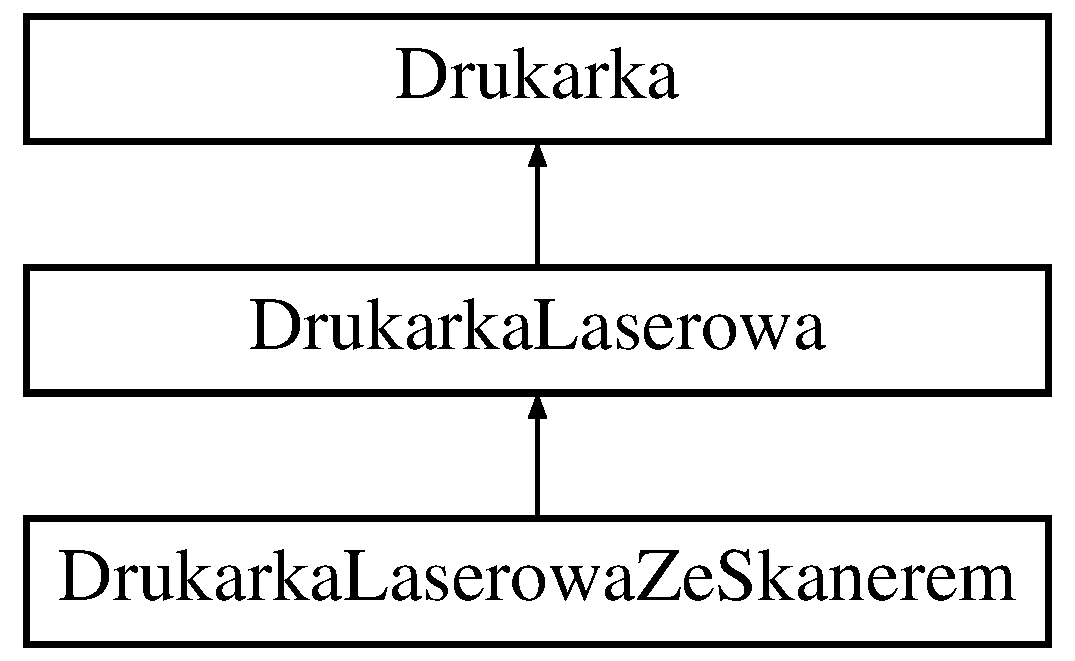
\includegraphics[height=3.000000cm]{class_drukarka_laserowa_ze_skanerem}
\end{center}
\end{figure}
\subsection*{Public Member Functions}
\begin{DoxyCompactItemize}
\item 
\textbf{ Drukarka\+Laserowa\+Ze\+Skanerem} ()
\begin{DoxyCompactList}\small\item\em Kontruktor domyslny. \end{DoxyCompactList}\item 
\textbf{ $\sim$\+Drukarka\+Laserowa\+Ze\+Skanerem} ()
\begin{DoxyCompactList}\small\item\em Destruktor. \end{DoxyCompactList}\item 
void \textbf{ zmien\+Parametry\+Urzadzenia} (int nowy\+\_\+parametr)
\begin{DoxyCompactList}\small\item\em Funkcja zmieniajaca wybrany parametr urzadzenia. \end{DoxyCompactList}\item 
void \textbf{ zapisz\+Urzadzenie} (\textbf{ Drukarka\+Laserowa\+Ze\+Skanerem} \&skaner)
\begin{DoxyCompactList}\small\item\em Zapisuje aktualne urzadzenie do pliku. \end{DoxyCompactList}\item 
void \textbf{ wczytaj\+Urzadzenie} (\textbf{ Drukarka\+Laserowa\+Ze\+Skanerem} \&skaner)
\begin{DoxyCompactList}\small\item\em Wczytuje aktualne urzadzenie z pliku. \end{DoxyCompactList}\item 
void \textbf{ wyswietl\+Rodzaj\+Drukarki} ()
\begin{DoxyCompactList}\small\item\em Funkcja wyswietlajaca rodzaj drukarki. \end{DoxyCompactList}\end{DoxyCompactItemize}
\subsection*{Friends}
\begin{DoxyCompactItemize}
\item 
std\+::ostream \& \textbf{ operator$<$$<$} (std\+::ostream \&s, \textbf{ Drukarka\+Laserowa\+Ze\+Skanerem} \&skaner)
\begin{DoxyCompactList}\small\item\em Operator strumieniowy $<$$<$. \end{DoxyCompactList}\item 
std\+::istream \& \textbf{ operator$>$$>$} (std\+::istream \&s, \textbf{ Drukarka\+Laserowa\+Ze\+Skanerem} \&skaner)
\begin{DoxyCompactList}\small\item\em Operator strumieniowy $>$$>$ \end{DoxyCompactList}\end{DoxyCompactItemize}
\subsection*{Additional Inherited Members}


\subsection{Detailed Description}
Klasa \doxyref{Drukarka\+Laserowa\+Ze\+Skanerem}{p.}{class_drukarka_laserowa_ze_skanerem}, pochodna klasy \doxyref{Drukarka\+Laserowa}{p.}{class_drukarka_laserowa}. 

\subsection{Constructor \& Destructor Documentation}
\mbox{\label{class_drukarka_laserowa_ze_skanerem_ada275234d6ac86c72babdbd7d929e5e2}} 
\index{Drukarka\+Laserowa\+Ze\+Skanerem@{Drukarka\+Laserowa\+Ze\+Skanerem}!Drukarka\+Laserowa\+Ze\+Skanerem@{Drukarka\+Laserowa\+Ze\+Skanerem}}
\index{Drukarka\+Laserowa\+Ze\+Skanerem@{Drukarka\+Laserowa\+Ze\+Skanerem}!Drukarka\+Laserowa\+Ze\+Skanerem@{Drukarka\+Laserowa\+Ze\+Skanerem}}
\subsubsection{Drukarka\+Laserowa\+Ze\+Skanerem()}
{\footnotesize\ttfamily Drukarka\+Laserowa\+Ze\+Skanerem\+::\+Drukarka\+Laserowa\+Ze\+Skanerem (\begin{DoxyParamCaption}{ }\end{DoxyParamCaption})}



Kontruktor domyslny. 

\mbox{\label{class_drukarka_laserowa_ze_skanerem_a41948d3844330a342d226e2ec2a4178c}} 
\index{Drukarka\+Laserowa\+Ze\+Skanerem@{Drukarka\+Laserowa\+Ze\+Skanerem}!````~Drukarka\+Laserowa\+Ze\+Skanerem@{$\sim$\+Drukarka\+Laserowa\+Ze\+Skanerem}}
\index{````~Drukarka\+Laserowa\+Ze\+Skanerem@{$\sim$\+Drukarka\+Laserowa\+Ze\+Skanerem}!Drukarka\+Laserowa\+Ze\+Skanerem@{Drukarka\+Laserowa\+Ze\+Skanerem}}
\subsubsection{$\sim$\+Drukarka\+Laserowa\+Ze\+Skanerem()}
{\footnotesize\ttfamily Drukarka\+Laserowa\+Ze\+Skanerem\+::$\sim$\+Drukarka\+Laserowa\+Ze\+Skanerem (\begin{DoxyParamCaption}{ }\end{DoxyParamCaption})}



Destruktor. 



\subsection{Member Function Documentation}
\mbox{\label{class_drukarka_laserowa_ze_skanerem_add71ac7e5ecf1cd4691c96b3e778e335}} 
\index{Drukarka\+Laserowa\+Ze\+Skanerem@{Drukarka\+Laserowa\+Ze\+Skanerem}!wczytaj\+Urzadzenie@{wczytaj\+Urzadzenie}}
\index{wczytaj\+Urzadzenie@{wczytaj\+Urzadzenie}!Drukarka\+Laserowa\+Ze\+Skanerem@{Drukarka\+Laserowa\+Ze\+Skanerem}}
\subsubsection{wczytaj\+Urzadzenie()}
{\footnotesize\ttfamily void Drukarka\+Laserowa\+Ze\+Skanerem\+::wczytaj\+Urzadzenie (\begin{DoxyParamCaption}\item[{\textbf{ Drukarka\+Laserowa\+Ze\+Skanerem} \&}]{skaner }\end{DoxyParamCaption})}



Wczytuje aktualne urzadzenie z pliku. 

\mbox{\label{class_drukarka_laserowa_ze_skanerem_aa37311823ae51a267ab614082ed38162}} 
\index{Drukarka\+Laserowa\+Ze\+Skanerem@{Drukarka\+Laserowa\+Ze\+Skanerem}!wyswietl\+Rodzaj\+Drukarki@{wyswietl\+Rodzaj\+Drukarki}}
\index{wyswietl\+Rodzaj\+Drukarki@{wyswietl\+Rodzaj\+Drukarki}!Drukarka\+Laserowa\+Ze\+Skanerem@{Drukarka\+Laserowa\+Ze\+Skanerem}}
\subsubsection{wyswietl\+Rodzaj\+Drukarki()}
{\footnotesize\ttfamily void Drukarka\+Laserowa\+Ze\+Skanerem\+::wyswietl\+Rodzaj\+Drukarki (\begin{DoxyParamCaption}{ }\end{DoxyParamCaption})\hspace{0.3cm}{\ttfamily [virtual]}}



Funkcja wyswietlajaca rodzaj drukarki. 



Reimplemented from \textbf{ Drukarka\+Laserowa} \doxyref{}{p.}{class_drukarka_laserowa_a6317c4138c4b0f5f26d7209aa9f6de86}.

\mbox{\label{class_drukarka_laserowa_ze_skanerem_a44a5fa9e498a6a695529865bcb541240}} 
\index{Drukarka\+Laserowa\+Ze\+Skanerem@{Drukarka\+Laserowa\+Ze\+Skanerem}!zapisz\+Urzadzenie@{zapisz\+Urzadzenie}}
\index{zapisz\+Urzadzenie@{zapisz\+Urzadzenie}!Drukarka\+Laserowa\+Ze\+Skanerem@{Drukarka\+Laserowa\+Ze\+Skanerem}}
\subsubsection{zapisz\+Urzadzenie()}
{\footnotesize\ttfamily void Drukarka\+Laserowa\+Ze\+Skanerem\+::zapisz\+Urzadzenie (\begin{DoxyParamCaption}\item[{\textbf{ Drukarka\+Laserowa\+Ze\+Skanerem} \&}]{skaner }\end{DoxyParamCaption})}



Zapisuje aktualne urzadzenie do pliku. 

\mbox{\label{class_drukarka_laserowa_ze_skanerem_af32643998dec727591bb3956074800b7}} 
\index{Drukarka\+Laserowa\+Ze\+Skanerem@{Drukarka\+Laserowa\+Ze\+Skanerem}!zmien\+Parametry\+Urzadzenia@{zmien\+Parametry\+Urzadzenia}}
\index{zmien\+Parametry\+Urzadzenia@{zmien\+Parametry\+Urzadzenia}!Drukarka\+Laserowa\+Ze\+Skanerem@{Drukarka\+Laserowa\+Ze\+Skanerem}}
\subsubsection{zmien\+Parametry\+Urzadzenia()}
{\footnotesize\ttfamily void Drukarka\+Laserowa\+Ze\+Skanerem\+::zmien\+Parametry\+Urzadzenia (\begin{DoxyParamCaption}\item[{int}]{nowy\+\_\+parametr }\end{DoxyParamCaption})\hspace{0.3cm}{\ttfamily [virtual]}}



Funkcja zmieniajaca wybrany parametr urzadzenia. 



Reimplemented from \textbf{ Drukarka\+Laserowa} \doxyref{}{p.}{class_drukarka_laserowa_aeb1c4870b0c7570a99992a694c7aebd1}.



\subsection{Friends And Related Function Documentation}
\mbox{\label{class_drukarka_laserowa_ze_skanerem_ab3d71d7a2059d279e4f7e3df02f89e5f}} 
\index{Drukarka\+Laserowa\+Ze\+Skanerem@{Drukarka\+Laserowa\+Ze\+Skanerem}!operator$<$$<$@{operator$<$$<$}}
\index{operator$<$$<$@{operator$<$$<$}!Drukarka\+Laserowa\+Ze\+Skanerem@{Drukarka\+Laserowa\+Ze\+Skanerem}}
\subsubsection{operator$<$$<$}
{\footnotesize\ttfamily std\+::ostream\& operator$<$$<$ (\begin{DoxyParamCaption}\item[{std\+::ostream \&}]{s,  }\item[{\textbf{ Drukarka\+Laserowa\+Ze\+Skanerem} \&}]{skaner }\end{DoxyParamCaption})\hspace{0.3cm}{\ttfamily [friend]}}



Operator strumieniowy $<$$<$. 

\mbox{\label{class_drukarka_laserowa_ze_skanerem_a664f0d835b6108a7be0b418d5a49c307}} 
\index{Drukarka\+Laserowa\+Ze\+Skanerem@{Drukarka\+Laserowa\+Ze\+Skanerem}!operator$>$$>$@{operator$>$$>$}}
\index{operator$>$$>$@{operator$>$$>$}!Drukarka\+Laserowa\+Ze\+Skanerem@{Drukarka\+Laserowa\+Ze\+Skanerem}}
\subsubsection{operator$>$$>$}
{\footnotesize\ttfamily std\+::istream\& operator$>$$>$ (\begin{DoxyParamCaption}\item[{std\+::istream \&}]{s,  }\item[{\textbf{ Drukarka\+Laserowa\+Ze\+Skanerem} \&}]{skaner }\end{DoxyParamCaption})\hspace{0.3cm}{\ttfamily [friend]}}



Operator strumieniowy $>$$>$ 



The documentation for this class was generated from the following files\+:\begin{DoxyCompactItemize}
\item 
Drukarka\+Laserowa cz.\+2/\textbf{ Drukarka\+Laserowa\+Ze\+Skanerem.\+h}\item 
Drukarka\+Laserowa cz.\+2/\textbf{ Drukarka\+Laserowa\+Ze\+Skanerem.\+cpp}\end{DoxyCompactItemize}

\section{Liczba\+Kartek Class Reference}
\label{class_liczba_kartek}\index{Liczba\+Kartek@{Liczba\+Kartek}}


Klasa \doxyref{Liczba\+Kartek}{p.}{class_liczba_kartek}, podklasa klasy \doxyref{Drukarka\+Laserowa}{p.}{class_drukarka_laserowa}.  




{\ttfamily \#include $<$Liczba\+Kartek.\+h$>$}

\subsection*{Public Member Functions}
\begin{DoxyCompactItemize}
\item 
\textbf{ Liczba\+Kartek} ()
\begin{DoxyCompactList}\small\item\em Kontruktor domyslny. \end{DoxyCompactList}\item 
\textbf{ $\sim$\+Liczba\+Kartek} ()
\begin{DoxyCompactList}\small\item\em destruktor \end{DoxyCompactList}\item 
void \textbf{ wyswietl\+Kartki} ()
\begin{DoxyCompactList}\small\item\em Funkcja wyswietlajaca aktualna ilosc kartek. \end{DoxyCompactList}\item 
void \textbf{ zmniejsz\+Kartki} ()
\begin{DoxyCompactList}\small\item\em Funkcja zmniejszajaca ilosc kartek. \end{DoxyCompactList}\item 
void \textbf{ wymiana\+Kartek} (int nowa\+\_\+ilosc\+\_\+kartek)
\begin{DoxyCompactList}\small\item\em Funkcja zmieniajaca ilosc kartek. \end{DoxyCompactList}\item 
void \textbf{ zapisz\+Urzadzenie} (\textbf{ Liczba\+Kartek} \&kartki)
\begin{DoxyCompactList}\small\item\em Zapisuje aktualne urzadzenie do pliku. \end{DoxyCompactList}\item 
void \textbf{ wczytaj\+Urzadzenie} (\textbf{ Liczba\+Kartek} \&kartki)
\begin{DoxyCompactList}\small\item\em Wczytuje aktualne urzadzenie z pliku. \end{DoxyCompactList}\end{DoxyCompactItemize}
\subsection*{Friends}
\begin{DoxyCompactItemize}
\item 
std\+::ostream \& \textbf{ operator$<$$<$} (std\+::ostream \&k, \textbf{ Liczba\+Kartek} \&kartki)
\begin{DoxyCompactList}\small\item\em Operator strumieniowy $<$$<$. \end{DoxyCompactList}\item 
std\+::istream \& \textbf{ operator$>$$>$} (std\+::istream \&k, \textbf{ Liczba\+Kartek} \&kartki)
\begin{DoxyCompactList}\small\item\em Operator strumieniowy $>$$>$ \end{DoxyCompactList}\end{DoxyCompactItemize}


\subsection{Detailed Description}
Klasa \doxyref{Liczba\+Kartek}{p.}{class_liczba_kartek}, podklasa klasy \doxyref{Drukarka\+Laserowa}{p.}{class_drukarka_laserowa}. 

\subsection{Constructor \& Destructor Documentation}
\mbox{\label{class_liczba_kartek_a5b8f9ef3090a1dda536258364fa0c98f}} 
\index{Liczba\+Kartek@{Liczba\+Kartek}!Liczba\+Kartek@{Liczba\+Kartek}}
\index{Liczba\+Kartek@{Liczba\+Kartek}!Liczba\+Kartek@{Liczba\+Kartek}}
\subsubsection{Liczba\+Kartek()}
{\footnotesize\ttfamily Liczba\+Kartek\+::\+Liczba\+Kartek (\begin{DoxyParamCaption}{ }\end{DoxyParamCaption})}



Kontruktor domyslny. 

\mbox{\label{class_liczba_kartek_a74b7c7c0734ae04ac8400d119ec73c2e}} 
\index{Liczba\+Kartek@{Liczba\+Kartek}!````~Liczba\+Kartek@{$\sim$\+Liczba\+Kartek}}
\index{````~Liczba\+Kartek@{$\sim$\+Liczba\+Kartek}!Liczba\+Kartek@{Liczba\+Kartek}}
\subsubsection{$\sim$\+Liczba\+Kartek()}
{\footnotesize\ttfamily Liczba\+Kartek\+::$\sim$\+Liczba\+Kartek (\begin{DoxyParamCaption}{ }\end{DoxyParamCaption})}



destruktor 



\subsection{Member Function Documentation}
\mbox{\label{class_liczba_kartek_adbe350d7e80efdd3485062f41c92efbe}} 
\index{Liczba\+Kartek@{Liczba\+Kartek}!wczytaj\+Urzadzenie@{wczytaj\+Urzadzenie}}
\index{wczytaj\+Urzadzenie@{wczytaj\+Urzadzenie}!Liczba\+Kartek@{Liczba\+Kartek}}
\subsubsection{wczytaj\+Urzadzenie()}
{\footnotesize\ttfamily void Liczba\+Kartek\+::wczytaj\+Urzadzenie (\begin{DoxyParamCaption}\item[{\textbf{ Liczba\+Kartek} \&}]{kartki }\end{DoxyParamCaption})}



Wczytuje aktualne urzadzenie z pliku. 

\mbox{\label{class_liczba_kartek_ac857fc73aff02972faa9563abc97bf7d}} 
\index{Liczba\+Kartek@{Liczba\+Kartek}!wymiana\+Kartek@{wymiana\+Kartek}}
\index{wymiana\+Kartek@{wymiana\+Kartek}!Liczba\+Kartek@{Liczba\+Kartek}}
\subsubsection{wymiana\+Kartek()}
{\footnotesize\ttfamily void Liczba\+Kartek\+::wymiana\+Kartek (\begin{DoxyParamCaption}\item[{int}]{nowa\+\_\+ilosc\+\_\+kartek }\end{DoxyParamCaption})}



Funkcja zmieniajaca ilosc kartek. 

\mbox{\label{class_liczba_kartek_a7642b71a3fa02723a13e7054da542b57}} 
\index{Liczba\+Kartek@{Liczba\+Kartek}!wyswietl\+Kartki@{wyswietl\+Kartki}}
\index{wyswietl\+Kartki@{wyswietl\+Kartki}!Liczba\+Kartek@{Liczba\+Kartek}}
\subsubsection{wyswietl\+Kartki()}
{\footnotesize\ttfamily void Liczba\+Kartek\+::wyswietl\+Kartki (\begin{DoxyParamCaption}{ }\end{DoxyParamCaption})}



Funkcja wyswietlajaca aktualna ilosc kartek. 

\mbox{\label{class_liczba_kartek_abc5adc55e7d13c0eb66497de259a1617}} 
\index{Liczba\+Kartek@{Liczba\+Kartek}!zapisz\+Urzadzenie@{zapisz\+Urzadzenie}}
\index{zapisz\+Urzadzenie@{zapisz\+Urzadzenie}!Liczba\+Kartek@{Liczba\+Kartek}}
\subsubsection{zapisz\+Urzadzenie()}
{\footnotesize\ttfamily void Liczba\+Kartek\+::zapisz\+Urzadzenie (\begin{DoxyParamCaption}\item[{\textbf{ Liczba\+Kartek} \&}]{kartki }\end{DoxyParamCaption})}



Zapisuje aktualne urzadzenie do pliku. 

\mbox{\label{class_liczba_kartek_a4290c8a40e540ea06570add9706f9e47}} 
\index{Liczba\+Kartek@{Liczba\+Kartek}!zmniejsz\+Kartki@{zmniejsz\+Kartki}}
\index{zmniejsz\+Kartki@{zmniejsz\+Kartki}!Liczba\+Kartek@{Liczba\+Kartek}}
\subsubsection{zmniejsz\+Kartki()}
{\footnotesize\ttfamily void Liczba\+Kartek\+::zmniejsz\+Kartki (\begin{DoxyParamCaption}{ }\end{DoxyParamCaption})}



Funkcja zmniejszajaca ilosc kartek. 



\subsection{Friends And Related Function Documentation}
\mbox{\label{class_liczba_kartek_a5d2f18a424b2dac713091623bd021ae0}} 
\index{Liczba\+Kartek@{Liczba\+Kartek}!operator$<$$<$@{operator$<$$<$}}
\index{operator$<$$<$@{operator$<$$<$}!Liczba\+Kartek@{Liczba\+Kartek}}
\subsubsection{operator$<$$<$}
{\footnotesize\ttfamily std\+::ostream\& operator$<$$<$ (\begin{DoxyParamCaption}\item[{std\+::ostream \&}]{k,  }\item[{\textbf{ Liczba\+Kartek} \&}]{kartki }\end{DoxyParamCaption})\hspace{0.3cm}{\ttfamily [friend]}}



Operator strumieniowy $<$$<$. 

\mbox{\label{class_liczba_kartek_a0bda24376dd794cf98b245fba9b685ce}} 
\index{Liczba\+Kartek@{Liczba\+Kartek}!operator$>$$>$@{operator$>$$>$}}
\index{operator$>$$>$@{operator$>$$>$}!Liczba\+Kartek@{Liczba\+Kartek}}
\subsubsection{operator$>$$>$}
{\footnotesize\ttfamily std\+::istream\& operator$>$$>$ (\begin{DoxyParamCaption}\item[{std\+::istream \&}]{k,  }\item[{\textbf{ Liczba\+Kartek} \&}]{kartki }\end{DoxyParamCaption})\hspace{0.3cm}{\ttfamily [friend]}}



Operator strumieniowy $>$$>$ 



The documentation for this class was generated from the following files\+:\begin{DoxyCompactItemize}
\item 
Drukarka\+Laserowa cz.\+2/\textbf{ Liczba\+Kartek.\+h}\item 
Drukarka\+Laserowa cz.\+2/\textbf{ Liczba\+Kartek.\+cpp}\end{DoxyCompactItemize}

\section{Parametry\+Urzadzenia Class Reference}
\label{class_parametry_urzadzenia}\index{Parametry\+Urzadzenia@{Parametry\+Urzadzenia}}


Klasa \doxyref{Parametry\+Urzadzenia}{p.}{class_parametry_urzadzenia}, podklasa klasy Drukatka\+Laserowa.  




{\ttfamily \#include $<$Parametry\+Urzadzenia.\+h$>$}

\subsection*{Public Member Functions}
\begin{DoxyCompactItemize}
\item 
\textbf{ Parametry\+Urzadzenia} ()
\begin{DoxyCompactList}\small\item\em Konstruktor domyslny. \end{DoxyCompactList}\item 
\textbf{ $\sim$\+Parametry\+Urzadzenia} ()
\begin{DoxyCompactList}\small\item\em Destruktor. \end{DoxyCompactList}\item 
void \textbf{ wyswietl\+Rodzaj\+Drukarki} ()
\begin{DoxyCompactList}\small\item\em Funkcja wyswietlajaca rodzaj drukarki. \end{DoxyCompactList}\item 
void \textbf{ zapisz\+Urzadzenie} (\textbf{ Parametry\+Urzadzenia} \&parametry)
\begin{DoxyCompactList}\small\item\em Zapisuje aktualne urzadzenie do pliku. \end{DoxyCompactList}\item 
void \textbf{ wczytaj\+Urzadzenie} (\textbf{ Parametry\+Urzadzenia} \&parametry)
\begin{DoxyCompactList}\small\item\em Wczytuje aktualne urzadzenie z pliku. \end{DoxyCompactList}\end{DoxyCompactItemize}
\subsection*{Friends}
\begin{DoxyCompactItemize}
\item 
std\+::ostream \& \textbf{ operator$<$$<$} (std\+::ostream \&p, \textbf{ Parametry\+Urzadzenia} \&parametry)
\begin{DoxyCompactList}\small\item\em Operator strumieniowy $<$$<$. \end{DoxyCompactList}\item 
std\+::istream \& \textbf{ operator$>$$>$} (std\+::istream \&p, \textbf{ Parametry\+Urzadzenia} \&parametry)
\begin{DoxyCompactList}\small\item\em Operator strumieniowy $>$$>$ \end{DoxyCompactList}\end{DoxyCompactItemize}


\subsection{Detailed Description}
Klasa \doxyref{Parametry\+Urzadzenia}{p.}{class_parametry_urzadzenia}, podklasa klasy Drukatka\+Laserowa. 

\subsection{Constructor \& Destructor Documentation}
\mbox{\label{class_parametry_urzadzenia_a7b592cadd35ada6c4f4829a0b9857d7e}} 
\index{Parametry\+Urzadzenia@{Parametry\+Urzadzenia}!Parametry\+Urzadzenia@{Parametry\+Urzadzenia}}
\index{Parametry\+Urzadzenia@{Parametry\+Urzadzenia}!Parametry\+Urzadzenia@{Parametry\+Urzadzenia}}
\subsubsection{Parametry\+Urzadzenia()}
{\footnotesize\ttfamily Parametry\+Urzadzenia\+::\+Parametry\+Urzadzenia (\begin{DoxyParamCaption}{ }\end{DoxyParamCaption})}



Konstruktor domyslny. 

\mbox{\label{class_parametry_urzadzenia_a7d4150d167a424076f625df9ed127a7e}} 
\index{Parametry\+Urzadzenia@{Parametry\+Urzadzenia}!````~Parametry\+Urzadzenia@{$\sim$\+Parametry\+Urzadzenia}}
\index{````~Parametry\+Urzadzenia@{$\sim$\+Parametry\+Urzadzenia}!Parametry\+Urzadzenia@{Parametry\+Urzadzenia}}
\subsubsection{$\sim$\+Parametry\+Urzadzenia()}
{\footnotesize\ttfamily Parametry\+Urzadzenia\+::$\sim$\+Parametry\+Urzadzenia (\begin{DoxyParamCaption}{ }\end{DoxyParamCaption})}



Destruktor. 



\subsection{Member Function Documentation}
\mbox{\label{class_parametry_urzadzenia_a311ad2b80a16f919f95144a15629e416}} 
\index{Parametry\+Urzadzenia@{Parametry\+Urzadzenia}!wczytaj\+Urzadzenie@{wczytaj\+Urzadzenie}}
\index{wczytaj\+Urzadzenie@{wczytaj\+Urzadzenie}!Parametry\+Urzadzenia@{Parametry\+Urzadzenia}}
\subsubsection{wczytaj\+Urzadzenie()}
{\footnotesize\ttfamily void Parametry\+Urzadzenia\+::wczytaj\+Urzadzenie (\begin{DoxyParamCaption}\item[{\textbf{ Parametry\+Urzadzenia} \&}]{parametry }\end{DoxyParamCaption})}



Wczytuje aktualne urzadzenie z pliku. 

\mbox{\label{class_parametry_urzadzenia_aea8b63aefeb940f08f37c21ab40d7224}} 
\index{Parametry\+Urzadzenia@{Parametry\+Urzadzenia}!wyswietl\+Rodzaj\+Drukarki@{wyswietl\+Rodzaj\+Drukarki}}
\index{wyswietl\+Rodzaj\+Drukarki@{wyswietl\+Rodzaj\+Drukarki}!Parametry\+Urzadzenia@{Parametry\+Urzadzenia}}
\subsubsection{wyswietl\+Rodzaj\+Drukarki()}
{\footnotesize\ttfamily void Parametry\+Urzadzenia\+::wyswietl\+Rodzaj\+Drukarki (\begin{DoxyParamCaption}{ }\end{DoxyParamCaption})}



Funkcja wyswietlajaca rodzaj drukarki. 

\mbox{\label{class_parametry_urzadzenia_a423f0ae8043db154ac78148840f6a95f}} 
\index{Parametry\+Urzadzenia@{Parametry\+Urzadzenia}!zapisz\+Urzadzenie@{zapisz\+Urzadzenie}}
\index{zapisz\+Urzadzenie@{zapisz\+Urzadzenie}!Parametry\+Urzadzenia@{Parametry\+Urzadzenia}}
\subsubsection{zapisz\+Urzadzenie()}
{\footnotesize\ttfamily void Parametry\+Urzadzenia\+::zapisz\+Urzadzenie (\begin{DoxyParamCaption}\item[{\textbf{ Parametry\+Urzadzenia} \&}]{parametry }\end{DoxyParamCaption})}



Zapisuje aktualne urzadzenie do pliku. 



\subsection{Friends And Related Function Documentation}
\mbox{\label{class_parametry_urzadzenia_aa482d2aa1e55c6e5d099eb3a47057d33}} 
\index{Parametry\+Urzadzenia@{Parametry\+Urzadzenia}!operator$<$$<$@{operator$<$$<$}}
\index{operator$<$$<$@{operator$<$$<$}!Parametry\+Urzadzenia@{Parametry\+Urzadzenia}}
\subsubsection{operator$<$$<$}
{\footnotesize\ttfamily std\+::ostream\& operator$<$$<$ (\begin{DoxyParamCaption}\item[{std\+::ostream \&}]{p,  }\item[{\textbf{ Parametry\+Urzadzenia} \&}]{parametry }\end{DoxyParamCaption})\hspace{0.3cm}{\ttfamily [friend]}}



Operator strumieniowy $<$$<$. 

\mbox{\label{class_parametry_urzadzenia_a3a936bf206691e70cd988e9db437769b}} 
\index{Parametry\+Urzadzenia@{Parametry\+Urzadzenia}!operator$>$$>$@{operator$>$$>$}}
\index{operator$>$$>$@{operator$>$$>$}!Parametry\+Urzadzenia@{Parametry\+Urzadzenia}}
\subsubsection{operator$>$$>$}
{\footnotesize\ttfamily std\+::istream\& operator$>$$>$ (\begin{DoxyParamCaption}\item[{std\+::istream \&}]{p,  }\item[{\textbf{ Parametry\+Urzadzenia} \&}]{parametry }\end{DoxyParamCaption})\hspace{0.3cm}{\ttfamily [friend]}}



Operator strumieniowy $>$$>$ 



The documentation for this class was generated from the following files\+:\begin{DoxyCompactItemize}
\item 
Drukarka\+Laserowa cz.\+2/\textbf{ Parametry\+Urzadzenia.\+h}\item 
Drukarka\+Laserowa cz.\+2/\textbf{ Parametry\+Urzadzenia.\+cpp}\end{DoxyCompactItemize}

\section{Poziom\+Tuszu Class Reference}
\label{class_poziom_tuszu}\index{Poziom\+Tuszu@{Poziom\+Tuszu}}


Klasa \doxyref{Poziom\+Tuszu}{p.}{class_poziom_tuszu}, podklasa klasy \doxyref{Drukarka\+Laserowa}{p.}{class_drukarka_laserowa}.  




{\ttfamily \#include $<$Poziom\+Tuszu.\+h$>$}

\subsection*{Public Member Functions}
\begin{DoxyCompactItemize}
\item 
\textbf{ Poziom\+Tuszu} ()
\begin{DoxyCompactList}\small\item\em Konstruktor domyslny. \end{DoxyCompactList}\item 
\textbf{ $\sim$\+Poziom\+Tuszu} ()
\begin{DoxyCompactList}\small\item\em Destruktor. \end{DoxyCompactList}\item 
void \textbf{ wyswietl\+Stan\+Tuszu} ()
\begin{DoxyCompactList}\small\item\em Funkcja wyswietlajaca stan tuszu. \end{DoxyCompactList}\item 
void \textbf{ zapisz\+Urzadzenie} (\textbf{ Poziom\+Tuszu} \&poziom)
\begin{DoxyCompactList}\small\item\em Zapisuje aktualne urzadzenie do pliku. \end{DoxyCompactList}\item 
void \textbf{ wczytaj\+Urzadzenie} (\textbf{ Poziom\+Tuszu} \&poziom)
\begin{DoxyCompactList}\small\item\em Wczytuje aktualne urzadzenie z pliku. \end{DoxyCompactList}\end{DoxyCompactItemize}
\subsection*{Friends}
\begin{DoxyCompactItemize}
\item 
std\+::ostream \& \textbf{ operator$<$$<$} (std\+::ostream \&t, \textbf{ Poziom\+Tuszu} \&poziom)
\begin{DoxyCompactList}\small\item\em Operator strumieniowy $<$$<$. \end{DoxyCompactList}\item 
std\+::istream \& \textbf{ operator$>$$>$} (std\+::istream \&t, \textbf{ Poziom\+Tuszu} \&poziom)
\begin{DoxyCompactList}\small\item\em Operator strumieniowy $>$$>$ \end{DoxyCompactList}\end{DoxyCompactItemize}


\subsection{Detailed Description}
Klasa \doxyref{Poziom\+Tuszu}{p.}{class_poziom_tuszu}, podklasa klasy \doxyref{Drukarka\+Laserowa}{p.}{class_drukarka_laserowa}. 

\subsection{Constructor \& Destructor Documentation}
\mbox{\label{class_poziom_tuszu_a53da3fdbb2342fedecefcf4fd620ae44}} 
\index{Poziom\+Tuszu@{Poziom\+Tuszu}!Poziom\+Tuszu@{Poziom\+Tuszu}}
\index{Poziom\+Tuszu@{Poziom\+Tuszu}!Poziom\+Tuszu@{Poziom\+Tuszu}}
\subsubsection{Poziom\+Tuszu()}
{\footnotesize\ttfamily Poziom\+Tuszu\+::\+Poziom\+Tuszu (\begin{DoxyParamCaption}{ }\end{DoxyParamCaption})}



Konstruktor domyslny. 

\mbox{\label{class_poziom_tuszu_a5bc03466d07b2c5397757eb2cb2d96b2}} 
\index{Poziom\+Tuszu@{Poziom\+Tuszu}!````~Poziom\+Tuszu@{$\sim$\+Poziom\+Tuszu}}
\index{````~Poziom\+Tuszu@{$\sim$\+Poziom\+Tuszu}!Poziom\+Tuszu@{Poziom\+Tuszu}}
\subsubsection{$\sim$\+Poziom\+Tuszu()}
{\footnotesize\ttfamily Poziom\+Tuszu\+::$\sim$\+Poziom\+Tuszu (\begin{DoxyParamCaption}{ }\end{DoxyParamCaption})}



Destruktor. 



\subsection{Member Function Documentation}
\mbox{\label{class_poziom_tuszu_ab714fbc75eabf40bd3b4a40906d2bee4}} 
\index{Poziom\+Tuszu@{Poziom\+Tuszu}!wczytaj\+Urzadzenie@{wczytaj\+Urzadzenie}}
\index{wczytaj\+Urzadzenie@{wczytaj\+Urzadzenie}!Poziom\+Tuszu@{Poziom\+Tuszu}}
\subsubsection{wczytaj\+Urzadzenie()}
{\footnotesize\ttfamily void Poziom\+Tuszu\+::wczytaj\+Urzadzenie (\begin{DoxyParamCaption}\item[{\textbf{ Poziom\+Tuszu} \&}]{poziom }\end{DoxyParamCaption})}



Wczytuje aktualne urzadzenie z pliku. 

\mbox{\label{class_poziom_tuszu_ada6bd40ebb881018e133b74d98661a8c}} 
\index{Poziom\+Tuszu@{Poziom\+Tuszu}!wyswietl\+Stan\+Tuszu@{wyswietl\+Stan\+Tuszu}}
\index{wyswietl\+Stan\+Tuszu@{wyswietl\+Stan\+Tuszu}!Poziom\+Tuszu@{Poziom\+Tuszu}}
\subsubsection{wyswietl\+Stan\+Tuszu()}
{\footnotesize\ttfamily void Poziom\+Tuszu\+::wyswietl\+Stan\+Tuszu (\begin{DoxyParamCaption}{ }\end{DoxyParamCaption})}



Funkcja wyswietlajaca stan tuszu. 

\mbox{\label{class_poziom_tuszu_a61c8d58febd5c511c5d2b60a7f048858}} 
\index{Poziom\+Tuszu@{Poziom\+Tuszu}!zapisz\+Urzadzenie@{zapisz\+Urzadzenie}}
\index{zapisz\+Urzadzenie@{zapisz\+Urzadzenie}!Poziom\+Tuszu@{Poziom\+Tuszu}}
\subsubsection{zapisz\+Urzadzenie()}
{\footnotesize\ttfamily void Poziom\+Tuszu\+::zapisz\+Urzadzenie (\begin{DoxyParamCaption}\item[{\textbf{ Poziom\+Tuszu} \&}]{poziom }\end{DoxyParamCaption})}



Zapisuje aktualne urzadzenie do pliku. 



\subsection{Friends And Related Function Documentation}
\mbox{\label{class_poziom_tuszu_a2335c59cd225161a0d7800e1a45ac3a9}} 
\index{Poziom\+Tuszu@{Poziom\+Tuszu}!operator$<$$<$@{operator$<$$<$}}
\index{operator$<$$<$@{operator$<$$<$}!Poziom\+Tuszu@{Poziom\+Tuszu}}
\subsubsection{operator$<$$<$}
{\footnotesize\ttfamily std\+::ostream\& operator$<$$<$ (\begin{DoxyParamCaption}\item[{std\+::ostream \&}]{t,  }\item[{\textbf{ Poziom\+Tuszu} \&}]{poziom }\end{DoxyParamCaption})\hspace{0.3cm}{\ttfamily [friend]}}



Operator strumieniowy $<$$<$. 

\mbox{\label{class_poziom_tuszu_ada6562c289860a5a222b70d7b83864c5}} 
\index{Poziom\+Tuszu@{Poziom\+Tuszu}!operator$>$$>$@{operator$>$$>$}}
\index{operator$>$$>$@{operator$>$$>$}!Poziom\+Tuszu@{Poziom\+Tuszu}}
\subsubsection{operator$>$$>$}
{\footnotesize\ttfamily std\+::istream\& operator$>$$>$ (\begin{DoxyParamCaption}\item[{std\+::istream \&}]{t,  }\item[{\textbf{ Poziom\+Tuszu} \&}]{poziom }\end{DoxyParamCaption})\hspace{0.3cm}{\ttfamily [friend]}}



Operator strumieniowy $>$$>$ 



The documentation for this class was generated from the following files\+:\begin{DoxyCompactItemize}
\item 
Drukarka\+Laserowa cz.\+2/\textbf{ Poziom\+Tuszu.\+h}\item 
Drukarka\+Laserowa cz.\+2/\textbf{ Poziom\+Tuszu.\+cpp}\end{DoxyCompactItemize}

\chapter{File Documentation}
\section{Drukarka\+Laserowa cz.2/\+Drukarka.cpp File Reference}
\label{_drukarka_8cpp}\index{Drukarka\+Laserowa cz.\+2/\+Drukarka.\+cpp@{Drukarka\+Laserowa cz.\+2/\+Drukarka.\+cpp}}
{\ttfamily \#include $<$iostream$>$}\newline
{\ttfamily \#include $<$string$>$}\newline
{\ttfamily \#include $<$fstream$>$}\newline
{\ttfamily \#include \char`\"{}Drukarka.\+h\char`\"{}}\newline
\subsection*{Functions}
\begin{DoxyCompactItemize}
\item 
std\+::ostream \& \textbf{ operator$<$$<$} (std\+::ostream \&d, \textbf{ Drukarka} \&drukarka)
\begin{DoxyCompactList}\small\item\em Zdefiniowany operator strumieniowy. \end{DoxyCompactList}\item 
std\+::istream \& \textbf{ operator$>$$>$} (std\+::istream \&d, \textbf{ Drukarka} \&drukarka)
\begin{DoxyCompactList}\small\item\em Zdefiniowany operator strumieniowy. \end{DoxyCompactList}\end{DoxyCompactItemize}


\subsection{Function Documentation}
\mbox{\label{_drukarka_8cpp_a82275125afd4c7b7e83ea20c28802918}} 
\index{Drukarka.\+cpp@{Drukarka.\+cpp}!operator$<$$<$@{operator$<$$<$}}
\index{operator$<$$<$@{operator$<$$<$}!Drukarka.\+cpp@{Drukarka.\+cpp}}
\subsubsection{operator$<$$<$()}
{\footnotesize\ttfamily std\+::ostream\& operator$<$$<$ (\begin{DoxyParamCaption}\item[{std\+::ostream \&}]{d,  }\item[{\textbf{ Drukarka} \&}]{drukarka }\end{DoxyParamCaption})}



Zdefiniowany operator strumieniowy. 

Operator strumieniowy $<$$<$. \mbox{\label{_drukarka_8cpp_a690d14a94727eaaeb482b4fa3356c761}} 
\index{Drukarka.\+cpp@{Drukarka.\+cpp}!operator$>$$>$@{operator$>$$>$}}
\index{operator$>$$>$@{operator$>$$>$}!Drukarka.\+cpp@{Drukarka.\+cpp}}
\subsubsection{operator$>$$>$()}
{\footnotesize\ttfamily std\+::istream\& operator$>$$>$ (\begin{DoxyParamCaption}\item[{std\+::istream \&}]{d,  }\item[{\textbf{ Drukarka} \&}]{drukarka }\end{DoxyParamCaption})}



Zdefiniowany operator strumieniowy. 

Operator strumieniowy $>$$>$ 
\section{Drukarka\+Laserowa cz.2/\+Drukarka.h File Reference}
\label{_drukarka_8h}\index{Drukarka\+Laserowa cz.\+2/\+Drukarka.\+h@{Drukarka\+Laserowa cz.\+2/\+Drukarka.\+h}}
{\ttfamily \#include $<$iostream$>$}\newline
{\ttfamily \#include $<$string$>$}\newline
{\ttfamily \#include $<$fstream$>$}\newline
\subsection*{Classes}
\begin{DoxyCompactItemize}
\item 
class \textbf{ Drukarka}
\begin{DoxyCompactList}\small\item\em Klasa abstrakcyjna. \end{DoxyCompactList}\end{DoxyCompactItemize}

\section{Drukarka\+Laserowa cz.2/\+Drukarka\+Atramentowa.cpp File Reference}
\label{_drukarka_atramentowa_8cpp}\index{Drukarka\+Laserowa cz.\+2/\+Drukarka\+Atramentowa.\+cpp@{Drukarka\+Laserowa cz.\+2/\+Drukarka\+Atramentowa.\+cpp}}
{\ttfamily \#include \char`\"{}Drukarka\+Atramentowa.\+h\char`\"{}}\newline
{\ttfamily \#include $<$iostream$>$}\newline
{\ttfamily \#include $<$string$>$}\newline
{\ttfamily \#include $<$fstream$>$}\newline
\subsection*{Functions}
\begin{DoxyCompactItemize}
\item 
std\+::ostream \& \textbf{ operator$<$$<$} (std\+::ostream \&a, \textbf{ Drukarka\+Atramentowa} \&atramentowa)
\begin{DoxyCompactList}\small\item\em Operator strumieniowy. \end{DoxyCompactList}\item 
std\+::istream \& \textbf{ operator$>$$>$} (std\+::istream \&a, \textbf{ Drukarka\+Atramentowa} \&atramentowa)
\begin{DoxyCompactList}\small\item\em Operator strumieniowy. \end{DoxyCompactList}\end{DoxyCompactItemize}
\subsection*{Variables}
\begin{DoxyCompactItemize}
\item 
string \textbf{ plik\+\_\+drukarka\+\_\+atramentowa} = \char`\"{}Drukarka\+Atramentowa.\+txt\char`\"{}
\begin{DoxyCompactList}\small\item\em Nazwa pliku do zapisu. \end{DoxyCompactList}\end{DoxyCompactItemize}


\subsection{Function Documentation}
\mbox{\label{_drukarka_atramentowa_8cpp_ad64f242b639e39ead86b549a16794760}} 
\index{Drukarka\+Atramentowa.\+cpp@{Drukarka\+Atramentowa.\+cpp}!operator$<$$<$@{operator$<$$<$}}
\index{operator$<$$<$@{operator$<$$<$}!Drukarka\+Atramentowa.\+cpp@{Drukarka\+Atramentowa.\+cpp}}
\subsubsection{operator$<$$<$()}
{\footnotesize\ttfamily std\+::ostream\& operator$<$$<$ (\begin{DoxyParamCaption}\item[{std\+::ostream \&}]{a,  }\item[{\textbf{ Drukarka\+Atramentowa} \&}]{atramentowa }\end{DoxyParamCaption})}



Operator strumieniowy. 

Operator strumieniowy $<$$<$. \mbox{\label{_drukarka_atramentowa_8cpp_ad81030cdd68ff1bd6990456164f9fe44}} 
\index{Drukarka\+Atramentowa.\+cpp@{Drukarka\+Atramentowa.\+cpp}!operator$>$$>$@{operator$>$$>$}}
\index{operator$>$$>$@{operator$>$$>$}!Drukarka\+Atramentowa.\+cpp@{Drukarka\+Atramentowa.\+cpp}}
\subsubsection{operator$>$$>$()}
{\footnotesize\ttfamily std\+::istream\& operator$>$$>$ (\begin{DoxyParamCaption}\item[{std\+::istream \&}]{a,  }\item[{\textbf{ Drukarka\+Atramentowa} \&}]{atramentowa }\end{DoxyParamCaption})}



Operator strumieniowy. 

Operator strumieniowy $>$$>$ 

\subsection{Variable Documentation}
\mbox{\label{_drukarka_atramentowa_8cpp_ab7f09af0ffaa32dae41ba70972c198bf}} 
\index{Drukarka\+Atramentowa.\+cpp@{Drukarka\+Atramentowa.\+cpp}!plik\+\_\+drukarka\+\_\+atramentowa@{plik\+\_\+drukarka\+\_\+atramentowa}}
\index{plik\+\_\+drukarka\+\_\+atramentowa@{plik\+\_\+drukarka\+\_\+atramentowa}!Drukarka\+Atramentowa.\+cpp@{Drukarka\+Atramentowa.\+cpp}}
\subsubsection{plik\+\_\+drukarka\+\_\+atramentowa}
{\footnotesize\ttfamily string plik\+\_\+drukarka\+\_\+atramentowa = \char`\"{}Drukarka\+Atramentowa.\+txt\char`\"{}}



Nazwa pliku do zapisu. 


\section{Drukarka\+Laserowa cz.2/\+Drukarka\+Atramentowa.h File Reference}
\label{_drukarka_atramentowa_8h}\index{Drukarka\+Laserowa cz.\+2/\+Drukarka\+Atramentowa.\+h@{Drukarka\+Laserowa cz.\+2/\+Drukarka\+Atramentowa.\+h}}
{\ttfamily \#include \char`\"{}Drukarka.\+h\char`\"{}}\newline
{\ttfamily \#include $<$iostream$>$}\newline
{\ttfamily \#include $<$string$>$}\newline
{\ttfamily \#include $<$fstream$>$}\newline
\subsection*{Classes}
\begin{DoxyCompactItemize}
\item 
class \textbf{ Drukarka\+Atramentowa}
\begin{DoxyCompactList}\small\item\em Klasa \doxyref{Drukarka\+Atramentowa}{p.}{class_drukarka_atramentowa}, pochodna klasy \doxyref{Drukarka}{p.}{class_drukarka}. \end{DoxyCompactList}\end{DoxyCompactItemize}

\section{Drukarka\+Laserowa cz.2/\+Drukarka\+Laserowa.cpp File Reference}
\label{_drukarka_laserowa_8cpp}\index{Drukarka\+Laserowa cz.\+2/\+Drukarka\+Laserowa.\+cpp@{Drukarka\+Laserowa cz.\+2/\+Drukarka\+Laserowa.\+cpp}}
{\ttfamily \#include \char`\"{}Drukarka\+Laserowa.\+h\char`\"{}}\newline
{\ttfamily \#include $<$iostream$>$}\newline
{\ttfamily \#include $<$string$>$}\newline
{\ttfamily \#include $<$fstream$>$}\newline
\subsection*{Functions}
\begin{DoxyCompactItemize}
\item 
std\+::ostream \& \textbf{ operator$<$$<$} (std\+::ostream \&l, \textbf{ Drukarka\+Laserowa} \&drukarka\+\_\+laserowa)
\begin{DoxyCompactList}\small\item\em Operator strumieniowy. \end{DoxyCompactList}\item 
std\+::istream \& \textbf{ operator$>$$>$} (std\+::istream \&l, \textbf{ Drukarka\+Laserowa} \&drukarka\+\_\+laserowa)
\begin{DoxyCompactList}\small\item\em Operator strumieniowy. \end{DoxyCompactList}\end{DoxyCompactItemize}
\subsection*{Variables}
\begin{DoxyCompactItemize}
\item 
string \textbf{ plik\+\_\+drukarka\+\_\+laserowa} = \char`\"{}Drukarka\+Laserowa.\+txt\char`\"{}
\begin{DoxyCompactList}\small\item\em Nazwa pliku do zapisu. \end{DoxyCompactList}\end{DoxyCompactItemize}


\subsection{Function Documentation}
\mbox{\label{_drukarka_laserowa_8cpp_a9aeecb5f56f3f86716b4668ba91803b9}} 
\index{Drukarka\+Laserowa.\+cpp@{Drukarka\+Laserowa.\+cpp}!operator$<$$<$@{operator$<$$<$}}
\index{operator$<$$<$@{operator$<$$<$}!Drukarka\+Laserowa.\+cpp@{Drukarka\+Laserowa.\+cpp}}
\subsubsection{operator$<$$<$()}
{\footnotesize\ttfamily std\+::ostream\& operator$<$$<$ (\begin{DoxyParamCaption}\item[{std\+::ostream \&}]{l,  }\item[{\textbf{ Drukarka\+Laserowa} \&}]{drukarka\+\_\+laserowa }\end{DoxyParamCaption})}



Operator strumieniowy. 

Operator strumieniowy $<$$<$. \mbox{\label{_drukarka_laserowa_8cpp_adab561874dc824b55c9695dd73b4cdff}} 
\index{Drukarka\+Laserowa.\+cpp@{Drukarka\+Laserowa.\+cpp}!operator$>$$>$@{operator$>$$>$}}
\index{operator$>$$>$@{operator$>$$>$}!Drukarka\+Laserowa.\+cpp@{Drukarka\+Laserowa.\+cpp}}
\subsubsection{operator$>$$>$()}
{\footnotesize\ttfamily std\+::istream\& operator$>$$>$ (\begin{DoxyParamCaption}\item[{std\+::istream \&}]{l,  }\item[{\textbf{ Drukarka\+Laserowa} \&}]{drukarka\+\_\+laserowa }\end{DoxyParamCaption})}



Operator strumieniowy. 

Operator strumieniowy $>$$>$ 

\subsection{Variable Documentation}
\mbox{\label{_drukarka_laserowa_8cpp_a2cd3bbbdddd1f1085587c64acf2a27df}} 
\index{Drukarka\+Laserowa.\+cpp@{Drukarka\+Laserowa.\+cpp}!plik\+\_\+drukarka\+\_\+laserowa@{plik\+\_\+drukarka\+\_\+laserowa}}
\index{plik\+\_\+drukarka\+\_\+laserowa@{plik\+\_\+drukarka\+\_\+laserowa}!Drukarka\+Laserowa.\+cpp@{Drukarka\+Laserowa.\+cpp}}
\subsubsection{plik\+\_\+drukarka\+\_\+laserowa}
{\footnotesize\ttfamily string plik\+\_\+drukarka\+\_\+laserowa = \char`\"{}Drukarka\+Laserowa.\+txt\char`\"{}}



Nazwa pliku do zapisu. 


\section{Drukarka\+Laserowa cz.2/\+Drukarka\+Laserowa.h File Reference}
\label{_drukarka_laserowa_8h}\index{Drukarka\+Laserowa cz.\+2/\+Drukarka\+Laserowa.\+h@{Drukarka\+Laserowa cz.\+2/\+Drukarka\+Laserowa.\+h}}
{\ttfamily \#include \char`\"{}Drukarka.\+h\char`\"{}}\newline
{\ttfamily \#include \char`\"{}Parametry\+Urzadzenia.\+h\char`\"{}}\newline
{\ttfamily \#include \char`\"{}Poziom\+Tuszu.\+h\char`\"{}}\newline
{\ttfamily \#include \char`\"{}Liczba\+Kartek.\+h\char`\"{}}\newline
{\ttfamily \#include $<$iostream$>$}\newline
{\ttfamily \#include $<$string$>$}\newline
{\ttfamily \#include $<$fstream$>$}\newline
\subsection*{Classes}
\begin{DoxyCompactItemize}
\item 
class \textbf{ Drukarka\+Laserowa}
\begin{DoxyCompactList}\small\item\em Klasa \doxyref{Drukarka\+Laserowa}{p.}{class_drukarka_laserowa}, pochodna klasy \doxyref{Drukarka}{p.}{class_drukarka}. \end{DoxyCompactList}\end{DoxyCompactItemize}

\section{Drukarka\+Laserowa cz.2/\+Drukarka\+Laserowa\+Ze\+Skanerem.cpp File Reference}
\label{_drukarka_laserowa_ze_skanerem_8cpp}\index{Drukarka\+Laserowa cz.\+2/\+Drukarka\+Laserowa\+Ze\+Skanerem.\+cpp@{Drukarka\+Laserowa cz.\+2/\+Drukarka\+Laserowa\+Ze\+Skanerem.\+cpp}}
{\ttfamily \#include $<$string$>$}\newline
{\ttfamily \#include $<$iostream$>$}\newline
{\ttfamily \#include $<$fstream$>$}\newline
{\ttfamily \#include \char`\"{}Drukarka\+Laserowa\+Ze\+Skanerem.\+h\char`\"{}}\newline
\subsection*{Functions}
\begin{DoxyCompactItemize}
\item 
std\+::ostream \& \textbf{ operator$<$$<$} (std\+::ostream \&s, \textbf{ Drukarka\+Laserowa\+Ze\+Skanerem} \&skaner)
\begin{DoxyCompactList}\small\item\em Zdefiniowany operator strumieniowy. \end{DoxyCompactList}\item 
std\+::istream \& \textbf{ operator$>$$>$} (std\+::istream \&s, \textbf{ Drukarka\+Laserowa\+Ze\+Skanerem} \&skaner)
\begin{DoxyCompactList}\small\item\em Zdefiniowany operator strumieniowy. \end{DoxyCompactList}\end{DoxyCompactItemize}
\subsection*{Variables}
\begin{DoxyCompactItemize}
\item 
string \textbf{ plik\+\_\+drukarka\+\_\+laserowa\+\_\+ze\+\_\+skanerem} = \char`\"{}Drukarka\+Laserowa\+Ze\+Skanerem.\+txt\char`\"{}
\begin{DoxyCompactList}\small\item\em Nazwa pliku do zapisu stanu. \end{DoxyCompactList}\end{DoxyCompactItemize}


\subsection{Function Documentation}
\mbox{\label{_drukarka_laserowa_ze_skanerem_8cpp_ab3d71d7a2059d279e4f7e3df02f89e5f}} 
\index{Drukarka\+Laserowa\+Ze\+Skanerem.\+cpp@{Drukarka\+Laserowa\+Ze\+Skanerem.\+cpp}!operator$<$$<$@{operator$<$$<$}}
\index{operator$<$$<$@{operator$<$$<$}!Drukarka\+Laserowa\+Ze\+Skanerem.\+cpp@{Drukarka\+Laserowa\+Ze\+Skanerem.\+cpp}}
\subsubsection{operator$<$$<$()}
{\footnotesize\ttfamily std\+::ostream\& operator$<$$<$ (\begin{DoxyParamCaption}\item[{std\+::ostream \&}]{s,  }\item[{\textbf{ Drukarka\+Laserowa\+Ze\+Skanerem} \&}]{skaner }\end{DoxyParamCaption})}



Zdefiniowany operator strumieniowy. 

Operator strumieniowy $<$$<$. \mbox{\label{_drukarka_laserowa_ze_skanerem_8cpp_a664f0d835b6108a7be0b418d5a49c307}} 
\index{Drukarka\+Laserowa\+Ze\+Skanerem.\+cpp@{Drukarka\+Laserowa\+Ze\+Skanerem.\+cpp}!operator$>$$>$@{operator$>$$>$}}
\index{operator$>$$>$@{operator$>$$>$}!Drukarka\+Laserowa\+Ze\+Skanerem.\+cpp@{Drukarka\+Laserowa\+Ze\+Skanerem.\+cpp}}
\subsubsection{operator$>$$>$()}
{\footnotesize\ttfamily std\+::istream\& operator$>$$>$ (\begin{DoxyParamCaption}\item[{std\+::istream \&}]{s,  }\item[{\textbf{ Drukarka\+Laserowa\+Ze\+Skanerem} \&}]{skaner }\end{DoxyParamCaption})}



Zdefiniowany operator strumieniowy. 

Operator strumieniowy $>$$>$ 

\subsection{Variable Documentation}
\mbox{\label{_drukarka_laserowa_ze_skanerem_8cpp_a955d601d2de0c93a4d90afb67ba024ea}} 
\index{Drukarka\+Laserowa\+Ze\+Skanerem.\+cpp@{Drukarka\+Laserowa\+Ze\+Skanerem.\+cpp}!plik\+\_\+drukarka\+\_\+laserowa\+\_\+ze\+\_\+skanerem@{plik\+\_\+drukarka\+\_\+laserowa\+\_\+ze\+\_\+skanerem}}
\index{plik\+\_\+drukarka\+\_\+laserowa\+\_\+ze\+\_\+skanerem@{plik\+\_\+drukarka\+\_\+laserowa\+\_\+ze\+\_\+skanerem}!Drukarka\+Laserowa\+Ze\+Skanerem.\+cpp@{Drukarka\+Laserowa\+Ze\+Skanerem.\+cpp}}
\subsubsection{plik\+\_\+drukarka\+\_\+laserowa\+\_\+ze\+\_\+skanerem}
{\footnotesize\ttfamily string plik\+\_\+drukarka\+\_\+laserowa\+\_\+ze\+\_\+skanerem = \char`\"{}Drukarka\+Laserowa\+Ze\+Skanerem.\+txt\char`\"{}}



Nazwa pliku do zapisu stanu. 


\section{Drukarka\+Laserowa cz.2/\+Drukarka\+Laserowa\+Ze\+Skanerem.h File Reference}
\label{_drukarka_laserowa_ze_skanerem_8h}\index{Drukarka\+Laserowa cz.\+2/\+Drukarka\+Laserowa\+Ze\+Skanerem.\+h@{Drukarka\+Laserowa cz.\+2/\+Drukarka\+Laserowa\+Ze\+Skanerem.\+h}}
{\ttfamily \#include \char`\"{}Drukarka\+Laserowa.\+h\char`\"{}}\newline
{\ttfamily \#include $<$iostream$>$}\newline
{\ttfamily \#include $<$string$>$}\newline
{\ttfamily \#include $<$fstream$>$}\newline
\subsection*{Classes}
\begin{DoxyCompactItemize}
\item 
class \textbf{ Drukarka\+Laserowa\+Ze\+Skanerem}
\begin{DoxyCompactList}\small\item\em Klasa \doxyref{Drukarka\+Laserowa\+Ze\+Skanerem}{p.}{class_drukarka_laserowa_ze_skanerem}, pochodna klasy \doxyref{Drukarka\+Laserowa}{p.}{class_drukarka_laserowa}. \end{DoxyCompactList}\end{DoxyCompactItemize}

\section{Drukarka\+Laserowa cz.2/\+Kompilacja.cpp File Reference}
\label{_kompilacja_8cpp}\index{Drukarka\+Laserowa cz.\+2/\+Kompilacja.\+cpp@{Drukarka\+Laserowa cz.\+2/\+Kompilacja.\+cpp}}
{\ttfamily \#include \char`\"{}Drukarka\+Laserowa.\+h\char`\"{}}\newline
{\ttfamily \#include \char`\"{}Drukarka\+Atramentowa.\+h\char`\"{}}\newline
{\ttfamily \#include \char`\"{}Drukarka\+Laserowa\+Ze\+Skanerem.\+h\char`\"{}}\newline
{\ttfamily \#include \char`\"{}Drukarka.\+h\char`\"{}}\newline
{\ttfamily \#include $<$iostream$>$}\newline
{\ttfamily \#include $<$string$>$}\newline
{\ttfamily \#include $<$vector$>$}\newline
\subsection*{Functions}
\begin{DoxyCompactItemize}
\item 
int \textbf{ main} ()
\begin{DoxyCompactList}\small\item\em Glowny program. \end{DoxyCompactList}\end{DoxyCompactItemize}
\subsection*{Variables}
\begin{DoxyCompactItemize}
\item 
string \textbf{ nowa\+\_\+nazwa}
\begin{DoxyCompactList}\small\item\em Zmienna przechowujaca nowa nazwe drukarki. \end{DoxyCompactList}\item 
string \textbf{ nowa\+\_\+marka}
\begin{DoxyCompactList}\small\item\em Zmienna przechowujaca nowa marke drukarki. \end{DoxyCompactList}\item 
int \textbf{ opcja}
\begin{DoxyCompactList}\small\item\em zmienna uzywana do wyboru opcji w menu \end{DoxyCompactList}\end{DoxyCompactItemize}


\subsection{Function Documentation}
\mbox{\label{_kompilacja_8cpp_ae66f6b31b5ad750f1fe042a706a4e3d4}} 
\index{Kompilacja.\+cpp@{Kompilacja.\+cpp}!main@{main}}
\index{main@{main}!Kompilacja.\+cpp@{Kompilacja.\+cpp}}
\subsubsection{main()}
{\footnotesize\ttfamily int main (\begin{DoxyParamCaption}{ }\end{DoxyParamCaption})}



Glowny program. 



\subsection{Variable Documentation}
\mbox{\label{_kompilacja_8cpp_abdc8622b0f8bafd694447c4770b1b10c}} 
\index{Kompilacja.\+cpp@{Kompilacja.\+cpp}!nowa\+\_\+marka@{nowa\+\_\+marka}}
\index{nowa\+\_\+marka@{nowa\+\_\+marka}!Kompilacja.\+cpp@{Kompilacja.\+cpp}}
\subsubsection{nowa\+\_\+marka}
{\footnotesize\ttfamily string nowa\+\_\+marka}



Zmienna przechowujaca nowa marke drukarki. 

\mbox{\label{_kompilacja_8cpp_ad5f5ff4a0299ecc44d218b6a04da19a5}} 
\index{Kompilacja.\+cpp@{Kompilacja.\+cpp}!nowa\+\_\+nazwa@{nowa\+\_\+nazwa}}
\index{nowa\+\_\+nazwa@{nowa\+\_\+nazwa}!Kompilacja.\+cpp@{Kompilacja.\+cpp}}
\subsubsection{nowa\+\_\+nazwa}
{\footnotesize\ttfamily string nowa\+\_\+nazwa}



Zmienna przechowujaca nowa nazwe drukarki. 

\mbox{\label{_kompilacja_8cpp_adaeb9433eaa673c6d8c4793b5bfd9ec3}} 
\index{Kompilacja.\+cpp@{Kompilacja.\+cpp}!opcja@{opcja}}
\index{opcja@{opcja}!Kompilacja.\+cpp@{Kompilacja.\+cpp}}
\subsubsection{opcja}
{\footnotesize\ttfamily int opcja}



zmienna uzywana do wyboru opcji w menu 


\section{Drukarka\+Laserowa cz.2/\+Liczba\+Kartek.cpp File Reference}
\label{_liczba_kartek_8cpp}\index{Drukarka\+Laserowa cz.\+2/\+Liczba\+Kartek.\+cpp@{Drukarka\+Laserowa cz.\+2/\+Liczba\+Kartek.\+cpp}}
{\ttfamily \#include \char`\"{}Liczba\+Kartek.\+h\char`\"{}}\newline
{\ttfamily \#include $<$iostream$>$}\newline
{\ttfamily \#include $<$string$>$}\newline
{\ttfamily \#include $<$fstream$>$}\newline
\subsection*{Functions}
\begin{DoxyCompactItemize}
\item 
std\+::ostream \& \textbf{ operator$<$$<$} (std\+::ostream \&k, \textbf{ Liczba\+Kartek} \&kartki)
\begin{DoxyCompactList}\small\item\em Zdefiniowany operator strumieniowy. \end{DoxyCompactList}\item 
std\+::istream \& \textbf{ operator$>$$>$} (std\+::istream \&k, \textbf{ Liczba\+Kartek} \&kartki)
\begin{DoxyCompactList}\small\item\em Zdefiniowany operator strumieniowy. \end{DoxyCompactList}\end{DoxyCompactItemize}
\subsection*{Variables}
\begin{DoxyCompactItemize}
\item 
string \textbf{ plik\+\_\+liczba\+\_\+kartek} = \char`\"{}Liczba\+Kartek.\+txt\char`\"{}
\begin{DoxyCompactList}\small\item\em Nazwa pliku do zapisu stanu obiektu. \end{DoxyCompactList}\end{DoxyCompactItemize}


\subsection{Function Documentation}
\mbox{\label{_liczba_kartek_8cpp_a5d2f18a424b2dac713091623bd021ae0}} 
\index{Liczba\+Kartek.\+cpp@{Liczba\+Kartek.\+cpp}!operator$<$$<$@{operator$<$$<$}}
\index{operator$<$$<$@{operator$<$$<$}!Liczba\+Kartek.\+cpp@{Liczba\+Kartek.\+cpp}}
\subsubsection{operator$<$$<$()}
{\footnotesize\ttfamily std\+::ostream\& operator$<$$<$ (\begin{DoxyParamCaption}\item[{std\+::ostream \&}]{k,  }\item[{\textbf{ Liczba\+Kartek} \&}]{kartki }\end{DoxyParamCaption})}



Zdefiniowany operator strumieniowy. 

Operator strumieniowy $<$$<$. \mbox{\label{_liczba_kartek_8cpp_a0bda24376dd794cf98b245fba9b685ce}} 
\index{Liczba\+Kartek.\+cpp@{Liczba\+Kartek.\+cpp}!operator$>$$>$@{operator$>$$>$}}
\index{operator$>$$>$@{operator$>$$>$}!Liczba\+Kartek.\+cpp@{Liczba\+Kartek.\+cpp}}
\subsubsection{operator$>$$>$()}
{\footnotesize\ttfamily std\+::istream\& operator$>$$>$ (\begin{DoxyParamCaption}\item[{std\+::istream \&}]{k,  }\item[{\textbf{ Liczba\+Kartek} \&}]{kartki }\end{DoxyParamCaption})}



Zdefiniowany operator strumieniowy. 

Operator strumieniowy $>$$>$ 

\subsection{Variable Documentation}
\mbox{\label{_liczba_kartek_8cpp_a00640b3c7deba569a02a8b469b6fa538}} 
\index{Liczba\+Kartek.\+cpp@{Liczba\+Kartek.\+cpp}!plik\+\_\+liczba\+\_\+kartek@{plik\+\_\+liczba\+\_\+kartek}}
\index{plik\+\_\+liczba\+\_\+kartek@{plik\+\_\+liczba\+\_\+kartek}!Liczba\+Kartek.\+cpp@{Liczba\+Kartek.\+cpp}}
\subsubsection{plik\+\_\+liczba\+\_\+kartek}
{\footnotesize\ttfamily string plik\+\_\+liczba\+\_\+kartek = \char`\"{}Liczba\+Kartek.\+txt\char`\"{}}



Nazwa pliku do zapisu stanu obiektu. 


\section{Drukarka\+Laserowa cz.2/\+Liczba\+Kartek.h File Reference}
\label{_liczba_kartek_8h}\index{Drukarka\+Laserowa cz.\+2/\+Liczba\+Kartek.\+h@{Drukarka\+Laserowa cz.\+2/\+Liczba\+Kartek.\+h}}
{\ttfamily \#include $<$fstream$>$}\newline
{\ttfamily \#include $<$iostream$>$}\newline
{\ttfamily \#include $<$string$>$}\newline
\subsection*{Classes}
\begin{DoxyCompactItemize}
\item 
class \textbf{ Liczba\+Kartek}
\begin{DoxyCompactList}\small\item\em Klasa \doxyref{Liczba\+Kartek}{p.}{class_liczba_kartek}, podklasa klasy \doxyref{Drukarka\+Laserowa}{p.}{class_drukarka_laserowa}. \end{DoxyCompactList}\end{DoxyCompactItemize}

\section{Drukarka\+Laserowa cz.2/\+Parametry\+Urzadzenia.cpp File Reference}
\label{_parametry_urzadzenia_8cpp}\index{Drukarka\+Laserowa cz.\+2/\+Parametry\+Urzadzenia.\+cpp@{Drukarka\+Laserowa cz.\+2/\+Parametry\+Urzadzenia.\+cpp}}
{\ttfamily \#include \char`\"{}Parametry\+Urzadzenia.\+h\char`\"{}}\newline
{\ttfamily \#include $<$iostream$>$}\newline
{\ttfamily \#include $<$string$>$}\newline
{\ttfamily \#include $<$fstream$>$}\newline
\subsection*{Functions}
\begin{DoxyCompactItemize}
\item 
std\+::ostream \& \textbf{ operator$<$$<$} (std\+::ostream \&p, \textbf{ Parametry\+Urzadzenia} \&parametry)
\begin{DoxyCompactList}\small\item\em Zdefiniowany operator strumieniowy. \end{DoxyCompactList}\item 
std\+::istream \& \textbf{ operator$>$$>$} (std\+::istream \&p, \textbf{ Parametry\+Urzadzenia} \&parametry)
\begin{DoxyCompactList}\small\item\em Zdefiniowany operator strumieniowy. \end{DoxyCompactList}\end{DoxyCompactItemize}
\subsection*{Variables}
\begin{DoxyCompactItemize}
\item 
string \textbf{ plik\+\_\+parametry\+\_\+urzadzenia} = \char`\"{}Parametry\+Urzadzenia.\+txt\char`\"{}
\begin{DoxyCompactList}\small\item\em Nazwa pliku do zapisu stanu obiektu. \end{DoxyCompactList}\end{DoxyCompactItemize}


\subsection{Function Documentation}
\mbox{\label{_parametry_urzadzenia_8cpp_aa482d2aa1e55c6e5d099eb3a47057d33}} 
\index{Parametry\+Urzadzenia.\+cpp@{Parametry\+Urzadzenia.\+cpp}!operator$<$$<$@{operator$<$$<$}}
\index{operator$<$$<$@{operator$<$$<$}!Parametry\+Urzadzenia.\+cpp@{Parametry\+Urzadzenia.\+cpp}}
\subsubsection{operator$<$$<$()}
{\footnotesize\ttfamily std\+::ostream\& operator$<$$<$ (\begin{DoxyParamCaption}\item[{std\+::ostream \&}]{p,  }\item[{\textbf{ Parametry\+Urzadzenia} \&}]{parametry }\end{DoxyParamCaption})}



Zdefiniowany operator strumieniowy. 

Operator strumieniowy $<$$<$. \mbox{\label{_parametry_urzadzenia_8cpp_a3a936bf206691e70cd988e9db437769b}} 
\index{Parametry\+Urzadzenia.\+cpp@{Parametry\+Urzadzenia.\+cpp}!operator$>$$>$@{operator$>$$>$}}
\index{operator$>$$>$@{operator$>$$>$}!Parametry\+Urzadzenia.\+cpp@{Parametry\+Urzadzenia.\+cpp}}
\subsubsection{operator$>$$>$()}
{\footnotesize\ttfamily std\+::istream\& operator$>$$>$ (\begin{DoxyParamCaption}\item[{std\+::istream \&}]{p,  }\item[{\textbf{ Parametry\+Urzadzenia} \&}]{parametry }\end{DoxyParamCaption})}



Zdefiniowany operator strumieniowy. 

Operator strumieniowy $>$$>$ 

\subsection{Variable Documentation}
\mbox{\label{_parametry_urzadzenia_8cpp_a54071ea6d499fcf94192a5f91421529d}} 
\index{Parametry\+Urzadzenia.\+cpp@{Parametry\+Urzadzenia.\+cpp}!plik\+\_\+parametry\+\_\+urzadzenia@{plik\+\_\+parametry\+\_\+urzadzenia}}
\index{plik\+\_\+parametry\+\_\+urzadzenia@{plik\+\_\+parametry\+\_\+urzadzenia}!Parametry\+Urzadzenia.\+cpp@{Parametry\+Urzadzenia.\+cpp}}
\subsubsection{plik\+\_\+parametry\+\_\+urzadzenia}
{\footnotesize\ttfamily string plik\+\_\+parametry\+\_\+urzadzenia = \char`\"{}Parametry\+Urzadzenia.\+txt\char`\"{}}



Nazwa pliku do zapisu stanu obiektu. 


\section{Drukarka\+Laserowa cz.2/\+Parametry\+Urzadzenia.h File Reference}
\label{_parametry_urzadzenia_8h}\index{Drukarka\+Laserowa cz.\+2/\+Parametry\+Urzadzenia.\+h@{Drukarka\+Laserowa cz.\+2/\+Parametry\+Urzadzenia.\+h}}
{\ttfamily \#include $<$string$>$}\newline
{\ttfamily \#include $<$iostream$>$}\newline
{\ttfamily \#include $<$fstream$>$}\newline
\subsection*{Classes}
\begin{DoxyCompactItemize}
\item 
class \textbf{ Parametry\+Urzadzenia}
\begin{DoxyCompactList}\small\item\em Klasa \doxyref{Parametry\+Urzadzenia}{p.}{class_parametry_urzadzenia}, podklasa klasy Drukatka\+Laserowa. \end{DoxyCompactList}\end{DoxyCompactItemize}

\section{Drukarka\+Laserowa cz.2/\+Poziom\+Tuszu.cpp File Reference}
\label{_poziom_tuszu_8cpp}\index{Drukarka\+Laserowa cz.\+2/\+Poziom\+Tuszu.\+cpp@{Drukarka\+Laserowa cz.\+2/\+Poziom\+Tuszu.\+cpp}}
{\ttfamily \#include \char`\"{}Poziom\+Tuszu.\+h\char`\"{}}\newline
{\ttfamily \#include $<$iostream$>$}\newline
{\ttfamily \#include $<$string$>$}\newline
{\ttfamily \#include $<$fstream$>$}\newline
{\ttfamily \#include $<$cstdlib$>$}\newline
\subsection*{Functions}
\begin{DoxyCompactItemize}
\item 
std\+::ostream \& \textbf{ operator$<$$<$} (std\+::ostream \&t, \textbf{ Poziom\+Tuszu} \&poziom)
\begin{DoxyCompactList}\small\item\em Zdefiniowany operator strumieniowy. \end{DoxyCompactList}\item 
std\+::istream \& \textbf{ operator$>$$>$} (std\+::istream \&t, \textbf{ Poziom\+Tuszu} \&poziom)
\begin{DoxyCompactList}\small\item\em Zdefiniowany operator strumieniowy. \end{DoxyCompactList}\end{DoxyCompactItemize}
\subsection*{Variables}
\begin{DoxyCompactItemize}
\item 
string \textbf{ plik\+\_\+poziom\+\_\+tuszu} = \char`\"{}Poziom\+Tuszu.\+txt\char`\"{}
\begin{DoxyCompactList}\small\item\em Nazwa pliku do zapisu stanu obiektu. \end{DoxyCompactList}\end{DoxyCompactItemize}


\subsection{Function Documentation}
\mbox{\label{_poziom_tuszu_8cpp_a2335c59cd225161a0d7800e1a45ac3a9}} 
\index{Poziom\+Tuszu.\+cpp@{Poziom\+Tuszu.\+cpp}!operator$<$$<$@{operator$<$$<$}}
\index{operator$<$$<$@{operator$<$$<$}!Poziom\+Tuszu.\+cpp@{Poziom\+Tuszu.\+cpp}}
\subsubsection{operator$<$$<$()}
{\footnotesize\ttfamily std\+::ostream\& operator$<$$<$ (\begin{DoxyParamCaption}\item[{std\+::ostream \&}]{t,  }\item[{\textbf{ Poziom\+Tuszu} \&}]{poziom }\end{DoxyParamCaption})}



Zdefiniowany operator strumieniowy. 

Operator strumieniowy $<$$<$. \mbox{\label{_poziom_tuszu_8cpp_ada6562c289860a5a222b70d7b83864c5}} 
\index{Poziom\+Tuszu.\+cpp@{Poziom\+Tuszu.\+cpp}!operator$>$$>$@{operator$>$$>$}}
\index{operator$>$$>$@{operator$>$$>$}!Poziom\+Tuszu.\+cpp@{Poziom\+Tuszu.\+cpp}}
\subsubsection{operator$>$$>$()}
{\footnotesize\ttfamily std\+::istream\& operator$>$$>$ (\begin{DoxyParamCaption}\item[{std\+::istream \&}]{t,  }\item[{\textbf{ Poziom\+Tuszu} \&}]{poziom }\end{DoxyParamCaption})}



Zdefiniowany operator strumieniowy. 

Operator strumieniowy $>$$>$ 

\subsection{Variable Documentation}
\mbox{\label{_poziom_tuszu_8cpp_aa8ffdcf14798d2542b3eb62cbfce754c}} 
\index{Poziom\+Tuszu.\+cpp@{Poziom\+Tuszu.\+cpp}!plik\+\_\+poziom\+\_\+tuszu@{plik\+\_\+poziom\+\_\+tuszu}}
\index{plik\+\_\+poziom\+\_\+tuszu@{plik\+\_\+poziom\+\_\+tuszu}!Poziom\+Tuszu.\+cpp@{Poziom\+Tuszu.\+cpp}}
\subsubsection{plik\+\_\+poziom\+\_\+tuszu}
{\footnotesize\ttfamily string plik\+\_\+poziom\+\_\+tuszu = \char`\"{}Poziom\+Tuszu.\+txt\char`\"{}}



Nazwa pliku do zapisu stanu obiektu. 


\section{Drukarka\+Laserowa cz.2/\+Poziom\+Tuszu.h File Reference}
\label{_poziom_tuszu_8h}\index{Drukarka\+Laserowa cz.\+2/\+Poziom\+Tuszu.\+h@{Drukarka\+Laserowa cz.\+2/\+Poziom\+Tuszu.\+h}}
{\ttfamily \#include $<$string$>$}\newline
{\ttfamily \#include $<$iostream$>$}\newline
{\ttfamily \#include $<$fstream$>$}\newline
\subsection*{Classes}
\begin{DoxyCompactItemize}
\item 
class \textbf{ Poziom\+Tuszu}
\begin{DoxyCompactList}\small\item\em Klasa \doxyref{Poziom\+Tuszu}{p.}{class_poziom_tuszu}, podklasa klasy \doxyref{Drukarka\+Laserowa}{p.}{class_drukarka_laserowa}. \end{DoxyCompactList}\end{DoxyCompactItemize}

%--- End generated contents ---

% Index
\backmatter
\newpage
\phantomsection
\clearemptydoublepage
\addcontentsline{toc}{chapter}{Index}
\printindex

\end{document}
